




%\section{Proof of  the Theorem 1}\label{appendix}
%%\setcounter{theorem}{2}
%
%
%% We   start by presenting  some  basic notations  and  formula.  
%
%For convenient reading, Theorem 1  is restated as follows:
%\setcounter{theorem}{0}
%\begin{theorem}\label{Theorem_optimal} 
%	Concerning  the  simplex case  for   model (1), there  exists one-to-one corrspondence between the  locally  maximized    skewness  directions  and    altitudes   from  a  vertex  to  the    sub-simplexes  constructed  by    the  left   $  n-1$   ones.
%\end{theorem}
%
%For  intuition,  the  structure  of the proof is   outlined  as  follows:
%\begin{itemize}
%		\item  in the Subsection  \ref{simp}, for the original model (1),  we first deduce  an equivalent model   via some derivations, which  is then our focus in the sequential analysis. 
%		
%	\item  in the Subsection  \ref{linkheight}, we       investigate the relationship between the altitudes of the simplex and the newly-reformulated  model, which is presented  in the Lemma \ref{Theorem_structure_altitude}. 
%	\item
%	  in the Subsection  \ref{station} -- \ref{locallymaximized}, we   deduce  the  structure  of  all these  locally  maximized  solutions  
%	  for the new model.
%	  Specifically, this is  done by  sequentially examining    the  first-order and  second-order    necessary condition     of the new model.   
%	  The results are summarized   in the Lemma \ref{Theorem_structureofall} and \ref{Theorem_structureoflocal}.  	
%	\item By combining the above  Lemma \ref{Theorem_structure_altitude}, \ref{Theorem_structureofall} and \ref{Theorem_structureoflocal},  we  finally finish the proof  of  the  main  Theorem \ref{Theorem_optimal}  in the  manuscript,  which is   completed   in  the     Subsection  \ref{prooftheorem1}.    	   
%\end{itemize}
%
%The details of each part are as follows. 





%\subsection{Simplication for Model (1)}\label{simp}


%\begin{remark}\label{proportion}
%	(\ref{propto_relation}) implies that 
%	the skewness for  $ \mathbf  R$  along the direction $\mathbf   w  $  
%	is proportional to the  third-order  and  second-order  
%	cumulant of $  \mathbf u^{\mathrm  T} $. 

	% Some   observations can be established from (\ref{propto_relation}) for the skewness of the simplex. 
	
	%And the superscript in $	\mathbf   u^{i} $ is to specify  the index of the vertex $\mathbf r_{i}$.
	
%	For the simplex with $n$ vectices and  altitudes, 
%	the corresponding  $  \mathbf u^{i}$   can be expressed as follows:
%	\begin{align}\label{altitudemat}
%	[\mathbf   u^{1}, \mathbf   u^{2}, \dots, \mathbf   u^{n}]
%	=
%	\left[\begin{array}{cccccc}
%	\eta    & \gamma  &  \gamma  & \cdots  & \gamma   & \gamma \\
%	\gamma  & \eta    & \gamma   & \cdots  & \gamma   & \gamma  \\
%	\gamma  & \gamma    & \eta   & \cdots  & \gamma   & \gamma  \\
%	\vdots  & \vdots  & \vdots   & \ddots  & \vdots   & \vdots \\
%	\gamma      & \gamma  &  \gamma  &  \cdots &  \eta   &  \gamma \\ 
%    \gamma      & \gamma  &  \gamma  &  \cdots & \gamma   & \eta
%	\end{array}\right].
%	\end{align}








%\begin{equation}\label{opti_ori}
%\begin{cases}
%\max\limits_{\mathbf w} \quad skew(\mathbf w^{\mathrm  T}\mathbf R)   \\
%\rm s.t. \quad \mathbf w^{\mathrm {T}}\mathbf w=1
%\end{cases},
%\end{equation}




%Clearly, due to  the equivalence between the original model (1) and  (\ref{optmodel}), 
%we  mainly  focus on  
%investigating  the    solutions  of  (\ref{optmodel}). 



% and   can be    not included  in it.
 


%There are some comments that are worth emphasizing. 
%Firstly, for different simplexes, the distribution of the vertices generally  differs.
%However, after the whiten operation, all these vertices will   lies in an  ball in ($n-1$)D space, which can be seen from   
%$  \frac  {1}{n}  \tilde {\mathbf R}  \tilde {\mathbf R}^{\mathrm T} =  \mathbf I_{n-1} $.
%This also indicates that all  the whiten simplexes become regular ones.
%Secondly, though for different simplexes, the distribution of the vertices in the ball may still  differ, they  are similar to each other, up to a rotation transformation.  
%This indicates that the form of $ \mathbf R$ and $\tilde {\mathbf R}$  is trivial, and   in the later analysis, we always assume  that the whiten regular simplex is a standard or unit $n-1$ one, whose  $n$ vertices form an identity matrix $ \mathbf I_{n}$.


%In  the  following,   we  will  focus  on  the model  (\ref{optmodel})   and proceed from two aspects:
%  one is the relation between the altitudes of the simplex with this model.
%the other  is   investigate  its  form of the locally maximized skewness solutions, 





%	\begin{equation}\label{opti_oriS}
%	\begin{cases}
%	\max\limits_{ \tilde {\mathbf v} } \quad \tilde {\mathcal S}  \tilde {\mathbf v}^{3}   \\
%	\rm s.t. \quad \tilde {\mathbf v}^{\mathrm {T}}\tilde {\mathbf v}=1
%	\end{cases}.
%	\end{equation}

\subsection{Optimization  theories of  Tensor eigenpairs}
In this part,  we briefly  introduce the  optimization theories   related to the tensor  eigenpairs problem. 
The  concept  of  tensor  eigenpairs  can be    understood  and  derived  by  considering  the  following   constrained  nonconvex optimization  model:
\begin{equation}\label{opti_ori}
\begin{cases}
\max\limits_{\mathbf v} \quad \mathcal S \mathbf v^{m}   \\
\rm s.t. \quad \mathbf v^{\mathrm {T}}\mathbf v=1
\end{cases}.
\end{equation}
The Lagrangian function 
of (\ref{opti_ori})  is  defined as:
\begin{equation}\label{Lagrangian_function}
L(\mathbf v, \lambda)=
\frac {1}  {\it m}
\mathcal S \mathbf v^{\it m}
+
\frac { \lambda} {2} (1-  \mathbf v^{\mathrm {T}}\mathbf v).
\end{equation}
When the gradient of
$  L(\mathbf v, \lambda) $ to
$ \mathbf  v $ is  $ \mathbf 0$,    the eigenpair of a  symmetric  tensor can  be  deduced,  which  was  independently    defined  by   Lim  and  Qi  in  2005:

\begin{definition} \cite{qi,lim} [\textbf{eigenpairs of  symmetric tensor}]
	Given a  tensor $\mathcal S   \in    T^{m}(\mathbb R^{n}) $,
	a pair
	$(\lambda ,\mathbf v )$
	is an  eigenpair  of  
	$\mathcal S  $ 
	if
	\begin{equation}\label{definition}
	%\begin{cases}
	\mathcal S \mathbf v^{m-1}=\lambda \mathbf v,
	%\end{cases}
	\end{equation}
	where
$ \lambda  \in  \mathbb C $
is  the  eigenvalue and
$ \mathbf v  \in   \mathbb C^{n \times  1} $
is the  corresponding   eigenvector   satisifying 
$\mathbf v^{\mathrm {T}}\mathbf v=1 $.
\end{definition}






The  first-order    gradient  derivation     (\ref{definition})   can be  used  to    obtain        all   stationary  points  of  (\ref{opti_ori}), i.e., 
all eigenpairs of tensor.   
Note  that   not all of the  stationary  points are  the  locally  optimal  points. 
Some of these    can be  categorized as the saddle points.  
While   the  second-order  derivation  information  plays  an  important  role  in  identifying    whether  a  stationary  point  is     locally    optimal   
or saddle  given    an  optimization   model.      The    second-order derivation  
of
$  L(\mathbf v, \lambda) $ 
to    $ \mathbf v $, which is  also  termed  the Hessian matrix of
(\ref{Lagrangian_function}),  is   denoted
by 
\begin{equation}\label{hessian_matrix}
\mathbf H(\mathbf v) = (m-1)\mathcal S \mathbf v^{m-2} - \lambda \mathbf I_{n-1} ,
\end{equation}
where
$\mathcal S \mathbf v^{m-2} $ was defined in Subsection \ref{notation},
and 
$ \mathbf I_{n-1} $
is an $ (n-1) \times (n-1) $  identity matrix.

Then,  
the 
locally    optimal   solutions of   (\ref{opti_ori})
can  be  identified  by
checking the  negative 
definiteness  
and determining the sign of each  eigenvalue
of the  following  matrix:
	\begin{align}\label{Mhess}
\mathbf {K}
& =  \mathbf  P_{\mathbf  v}^{\bot} \mathbf H (\mathbf v)   \mathbf  P_{\mathbf  v}^{\bot}
	\end{align}
	and the  detailed  explanation for  the  
	derivation of 
	(\ref{Mhess})
	can refer to the Appendix part. 
	
	




%\begin{lemma}\label{phequal}  
%	Let  $\mathbf  u	\in \mathbb R^{n\times  1} $   and  $  \mathbf P = 
%	\mathbf Q_{2}^{\mathrm T}
%	\mathbf H(\mathbf u) 
%	\mathbf Q_{2} 
%	\in \mathbb R^{(n-1) \times  (n-1)} 
%	$  be   the  projected  Hessian  matrix   at  the  point    $\mathbf  u$,  where  $\mathbf H(\mathbf u) $  is  defined  in  (\ref{hessian_matrix}), and    $ \mathbf Q_{2}$ is  calculated  by  (\ref{QR_factor}). 
%	Define  a  new  matrix 
%	$  \mathbf {M}=  \mathbf  P_{\mathbf  u}^{\bot} \mathbf H (\mathbf u) 
%	\mathbf  P_{\mathbf  u}^{\bot}   $,
%	where   
%	$  \mathbf  P_{\mathbf  u}^{\bot} $ is the orthogonal  \textcolor{blue}{complement}   projector  of   $\mathbf u$.
%	Then,  it     holds  
%	\begin{equation}
%	\mathbf P   \preceq 0
%	\quad 
%	\Leftrightarrow
%	\quad 
%	\mathbf {M}  \preceq 0.	
%	\end{equation} 	  
%\end{lemma}


%	\subsection{Robust  eigenpairs of  symmetric tensors}\label{robustsection}
%	
%	One of  the  widely used  algorithms  to  obtain  tensor   eigenpairs  is  called  the  tensor  power   method, which 
%	is  based on  the  following  mapping  function   
%	\begin{equation}
%	\phi(\mathbf{v})=\frac{\mathcal S  \mathbf{v}^{m-1}}{\left\|\mathcal S  \mathbf{v}^{m-1}\right\|}
%	\end{equation}
%and  performs  the  following  iterative  schedule:	
%	\begin{equation}\label{tenpower}
%	\mathbf  {v}_{k+1} \mapsto \frac{\mathcal{S}  \mathbf{v}_{k}^{m-1}}{\left\|\mathcal{S}  \mathbf{v}_{k}^{m-1}\right\|}
%	.
%	\end{equation}
%	Given  a random   initialization  vector  
%	$ 	\mathbf  {v}_{0} $
%	and  iterate the above  formula 
%	(\ref{tenpower}) until  some  termination condition  is  satisfied,  an  eigenpair  can be  obtained. 
%	Then,  a   robust eigenvector of $ \mathcal{S} $  is an eigenvector  $  \mathbf v $ that is an attracting
%	fixed point of the tensor power method, 
%which 
%	can be identified  by  calculating  the spectral radius of the Jacobian  matirx   of  the  map  function,  which  is   denoted  and  given  by 	
%	\begin{equation}\label{Jacobianmatirx} 
%	\mathbf{J}  := \mathbf{J}(\mathbf{v})=\frac{m-1}{\lambda}\left(\mathcal{S}  \mathbf{v}^{m-2}- \lambda  \mathbf{v} \mathbf{v}^{\top}\right)
%	\end{equation}
%	
%	If the  spectral  radius  of  $  	\mathbf{J}(\mathbf{v}) $ is  less than  1,  it  is  said  that  the  corresponding  eigenpair  is  a  robust  one. 
%The  detailed derivations  can  refer  to 
%the  Lemmas 3.2 and 3.3  in \cite{RobustEigen}.

	
		\subsection{Regular  simplex  frame  and  tensor}
		In this part,  we  will  introduce  a  special class of symmetric   tensors,  which is termed   
		regular  simplex  one. 
		First,  the    definition of the  generalized  equiangular set  is  introduced as  follows:  
		\begin{definition}[Definition 4.1  in Ref. \cite{RobustEigen}]
		An equiangular set (ES) is a collection of vectors $\mathbf{w}_{1}, \ldots, \mathbf{w}_{r} \in \mathbb{R}^{n-1}$ with $r \geq n-1$ if there exists $\alpha \in \mathbb{R}$ such that
		$$
		\alpha=
		\left|\left\langle\mathbf{w}_{i}, \mathbf{w}_{j}\right\rangle\right|, \forall i \neq j \quad \text { and } \quad\left\|\mathbf{w}_{i}\right\|=1, \forall i .
		$$
		Furthermore, an $\mathrm{ES}$ is  called  an equiangular tight frame (ETF)  if  
		\begin{equation}
	\mathbf{W} \mathbf{W}^{\mathrm T}=a \mathbf{I}_{(n-1)}, \quad \mathbf{W}:=\left(\mathbf{w}_{1},  \cdots,  \mathbf{w}_{r}\right) \in \mathbb{R}^{(n-1) \times r}
	\end{equation}
	\end{definition}
	
		
	For  example, 
	when   $r=n-1$ and $a=1$, the  orthonormal bases
	 $\left\{\mathbf{w}_{1}, \ldots, \mathbf{w}_{n-1}\right\} \subset \mathbb{R}^{(n-1) \times (n-1)}$
	 forms  an  ETF,  where $\alpha =0$.
	 When    $r=n$ and $a=\frac {n}{n-1}$,   $\left\{\mathbf{w}_{1}, \ldots, \mathbf{w}_{n}\right\} \subset \mathbb{R}^{(n-1) \times  n}$, it  is   termed  
	 regular  simplex frames,  
	 where   $ 
	 \alpha = - \frac{1}{n-1}$.
	 $\mathbf{w}_{i}, i=1,2 \dots, n$   are  called  the  vectors  in  the  frame. 
	 In  2D  space,  
	 the  regular simplex  frame  is  a   regular  triangle.

	 
	 
	 In  addition, for the regular  simplex frame,  the  following property  holds,  which  will be  useful in  the  later  section: 
	 
	 \begin{property}\label{regularproperty}
	For  the  regular  simplex   frame,  the nullspace of 
	 $ \mathbf{W}^{\mathrm T} \mathbf{W} $
	  and 	 $  \mathbf{W} $
	   is spanned by 
	   $ \mathbf{1}_{n} $,
	   i.e., 
	    $ 
	    \mathbf{W}^{\mathrm T} \mathbf{W}  \mathbf{1}_{n} 
	    =
	     \mathbf{W}  \mathbf{1}_{n} 
	     =
	     \mathbf{0}_{n-1}
	    $.
	    %	 In  addition, it also holds that 
	   	 \end{property}
		
		
		Then,  the  regular  simplex  tensor  is   one  deduced  by  the  the  regular  simplex   frame  with  the  following   form:
		\begin{equation}\label{simplextensor}
		\mathcal{S}:=\sum_{i=1}^{n} \mathbf{w}_{i}^{\circ m}
		\end{equation}
		where $\circ$ is the outer product  defined  in Definition \ref{outerprod}, 
and  	$\mathcal{S}
	$ is  a   symmetric  tensor of order
		$ m $
		and dimension
		$ n-1$.   
		Note that
		when the tensor is generated by the orthonormal bases
		$\left\{\mathbf{w}_{1}, \ldots, \mathbf{w}_{n-1}\right\} \subset \mathbb{R}^{(n-1) \times (n-1)}$,
		the corresponding tensor is called an orthogonally  decomposable (odeco).
		Clearly, the regular simplex tensor can be viewed as a generalization of the odeco tensors. 
	
	
%		\subsection{Main Result}\label{MainResult}
%		%This part mainly  	
%			In  this  paper,  we   mainly  analyze  the  robust  eigenpairs  of  regular  simplex  tensor  and  focus on   the  following  conjecture:  % originally  presented  in  Ref  \cite{RobustEigen}:
%	\begin{conjecture}[Conjecture 4.7 in  Ref  \cite{RobustEigen} ] \label{conjecturesimplex}
%			The robust eigenvectors of a regular simplex tensor   are precisely the
%			vectors in the frame.
%		\end{conjecture}	
%	
%This  conjecture 
%	was originally  proposed in \cite{RobustEigen}.
%	Later, several researchers  also  considered this problem  in \cite{teneigenstructure}. 
%	They  investigated  the  real  eigen-structure of  such a type of tensor  
%	as well as the robustness of eigenpairs. 
%	However, they only provided the robustness proof for the case of  $n=3$,
%	and the experimental results for  the case  of   $n=4$.
%	To  our  best  knowledge,  so far, 
%	these  references are the only two works 
%	focusing on  identifying  the  robust  eigenpairs of regular  simplex  tensor. 
%	In this paper, we proceed further concerning the above  conjecture and make some progresses.
%	Our main contribution in this  paper can be summarized as the  following  theorem:
%		\begin{theorem}\label{maintheorem}
%	For  a regular simplex tensor,    all   the
%		vectors in the frame  are the robust ones. 
%	\end{theorem}	
%
%Note that the  conclusion in the above theorem \ref{maintheorem} 
% is a    relatively weaker one compared to that in the   original conjecture  4.7. 
% Theorem \ref{maintheorem}  
% only shows  the existence of the robust eigenpairs, and 
%demonstrate that  all   the
% vectors in the frame  are indeed the robust ones. 
% However, 
% it still  does not  justify  concerning  the conjecture that  the robust eigenpairs  
% are only these vectors in the frame. 
% 
% %\begin{remark}
% [\textbf{The outline of the proof}]
% To  prove Theorem \ref{maintheorem}, and for a better organization of the proof outline, 
% the  conclusion  is  further  decomposed into the following  two 
%steps:
% 	\begin{itemize}		
% 	\item  We  first  prove that 
%    all   the
% 	vectors in the frame  are  eigenpairs  	of  a regular simplex tensor, 
% 	which is proved in 
% 	Section  \ref{station}.
% 	\item  Then,  we  show  that  
% all   these 
%vectors in the frame  are  also   robust,
%which is proved in 
%Section   \ref{locallymaximized}
%
%\end{itemize}
%
%For  the  first  step,  
%we need to analyze the eigen-structure of all  eigenpairs,  and  to 
%prove that 
% all   the
%vectors in the frame  is  a  subset  of  all  eigenpairs. 
%Note that although this has been  done in previous Ref \cite{teneigenstructure}, 
%our proof outline  adopted in this paper is  different  from that in  \cite{teneigenstructure}, and the comparison 
% is  listed in Table \ref{tableforcomparison}.
%For  the  second  step,  
%directly  calculating the Jacobian matrix  and  
%determining the spectral radius  
%is also  difficult,  which  has been done in the previous work \cite{teneigenstructure}
%and only the case of $n=3$ can be analyzed.
%To deal with this problem, in the following section,  we develop 
%an auxiliary  criterion for the robustness identification  of   these  vectors  in the frame, and the details are presented in 
%Subsection  \ref{NewCriterion}.
%% \end{remark}

 
In  this paper, 
we will mainly focus on such a type of 	 
regular simplex tensor and tend to  analyze its eigen-stucture, including its stationary and locally optimal solutions. 
Before our discussion,	some necessary remarks   concerning  the discussed  scope    are  made as follows:
	\begin{remark}\label{RemarkScope}
		
		\begin{itemize}
			\item The notation  adopted   in this paper  is slightly  different from the previous work \cite{RobustEigen,teneigenstructure}.
			The existing ones considered  $n+1$ vertices in $n $ dimensional space, while  here we
			considered  $n$ vertices in $n-1 $ dimensional space. 
			Such a  modification is done for a convenient  formula  derivations  in the later  section (see Section  \ref{reformulated} for details), which is  trivial.
				\item 
				Throughout this paper,  we  only  concern with the case where 
				$n \ge 3, m \ge 3$  for (\ref{simplextensor}). 
				The matrix case (corresponding to 	$ m = 2$)  was not included in the discussion, since it can be checked that 
				when $m=2$, the second-order tensor for (\ref{simplextensor}) will be 
				proportional to an  identity matrix, up to a constant factor, whose  eigen-structure is  obvious.
				In addition,  it should also be noted that 
				the case  of 		$n = 3, m = 4$   turns to be  a very  special combination, 
				whose corresponding   objective  value, i.e., 
				$
			\mathcal S \mathbf v^{m}, 
			$   is a constant.
				Such a  conclusion has been analyzed in Theorem 4.6 of \cite{RobustEigen}  
				 and Theorem 12 of \cite{teneigenstructure}.
				Please refer for  details. 		
				In the later analysis, 
				this combination is also always excluded out of the discussed scope. 	
		\end{itemize}
	\end{remark}
		
% \subsection{Relation between  altitude of simplex and  model (\ref{optmodel})}\label{linkheight}


\section{Problem  reformulation for   regular simplex  tensor eigenpairs}\label{reformulated}

%In  this  part,  we  focus  on    the  above  Conjecture   \ref{conjecturesimplex} and tend to  prove 
%our presented Theorem \ref{maintheorem}. 
%To  deal  with  this   problem,  
In  this  part, we   first  transform  the  optimization  model     by  
reformulating  a  new  model  for  the  regular  simplex  tensor.
The  details are as  follows.

 %\subsection{Model  Reformulation  for  regular  simplex  tensor}\label{Simpleillustration}
 Directly  focusing  on  the  original  optimization model   (\ref{opti_ori}) where  the  tensor  is  given  by  (\ref{simplextensor})
 may be  a  complicated   task.
 In  this  part,  by  utilizing  
 Property  \ref{regularproperty}, 
 an equivalent   optimization  model  is  reformulated  to   deal  with  the  issue. 
% The  details  are  as  follows.
 First,  
 the  objective function   when $ \mathcal{S}$ is  given by  (\ref{simplextensor}) can be  rewritten as:
 	\begin{equation}
 \mathcal{S}  \mathbf v^{m}    
  =
 (\sum_{i=1}^{n} \mathbf{w}_{i}^{\circ m} )\mathbf v^{m} 
 =
  \sum_{i=1}^{n} ( \mathbf v^{\mathrm T} \mathbf{w}_{i})^{ m} .
 \end{equation}
 Denote  
 \begin{align}\label{udenote}
 \mathbf   u =
 \sqrt {
 	  \frac  {n-1}{ n}
  }   
 {\mathbf W}^{\mathrm T}  {\mathbf v}  = 
 [u_1,u_2,\dots, u_{n}]^{\mathrm T} \in  \mathbb {R}^{n \times 1} ,
 \end{align} 
 it holds that
 	\begin{equation}
 \mathcal{S}  \mathbf v^{m}    
\varpropto 
\sum\limits_{i=1}^{n}  u_{i}^{m}.
 \end{equation}
Furthermore, 
we  can  derive  that 
  \begin{align}\label{utu}
 \mathbf   u ^{\mathrm T} \mathbf   u
  =
   \frac  {n-1}{  n  }  
   {\mathbf v} ^{\mathrm T} {\mathbf W} {\mathbf W}^{\mathrm T}  {\mathbf v}  
   =
   {\mathbf v} ^{\mathrm T}  {\mathbf v}  
   =1 ,
 \end{align}
 and 
   \begin{align}\label{uln}
 \mathbf   u ^{\mathrm T}
  \mathbf 1_{n}
 =
 \sqrt {
	\frac  {n-1}{ n}
}   
 {\mathbf v} ^{\mathrm T} {\mathbf W}   {\mathbf 1_{n}}  
 = 
0 .
 \end{align}
 
Then,  model   (\ref{opti_ori})   for the regular simplex tensor, which is with the following form 
 \begin{align}\label{optmodelori}
\begin{cases}
\max\limits_{\mathbf v} \quad \mathcal S \mathbf v^{m} 
=
(\sum\limits_{i=1}^{n} \mathbf{w}_{i}^{\circ m}) \mathbf v^{m}   \\
\rm s.t. \quad \mathbf v^{\mathrm {T}}\mathbf v=1
\end{cases}
\end{align}
  can  be  equivalently    transformed into the following 
 model:  
 \begin{align}\label{optmodel}
 \begin{cases}
 \max\limits_{\mathbf u}  \quad  \sum\limits_{i=1}^{n}  u_{i}^{m} 
  \\
 \text { s.t. }   \quad    
 \mathbf   u^{\mathrm T}   \mathbf   u =1 ,
 \quad  
 \mathbf   u^{\mathrm T}   \mathbf   1_{n} =0
 \end{cases} .
 \end{align}
 
% when $m=4$ and $n=3$,  
% due  to  the constraint  
%$  \mathbf   u^{\mathrm T}   \mathbf   u =1 $ , 
% we can set 
% $ 
% u_{1} = cos (\theta_{1}),
% u_{2} = cos (\theta_{1}) cos (\theta_{2}),
% u_{3} =  cos (\theta_{1}) sin (\theta_{2})
% $
% 
%  \begin{align}%\label{optmodel}
%  \sum\limits_{i=1}^{n}  u_{i}^{m}  
%  =
%  cos^{4} (\theta_{1})
%  +
%  cos ^{4}(\theta_{1}) cos^{4} (\theta_{2})
%  +
%   cos^{4} (\theta_{1}) sin^{4} (\theta_{2})
% \end{align}
% 
% 
%   \begin{align}%\label{optmodel}
%(  u_{1}^{2} +   u_{2}^{2}+    u_{3}^{2}  )
%(  u_{1}^{2} +   u_{3}^{2}+    u_{3}^{2}  )
% =
%   \sum\limits_{i=1}^{n}  u_{i}^{4}  
%   +
% 2u_{1}^{2}      u_{2}^{2}  
%    +
% 2u_{1}^{2}      u_{3}^{2} 
%    +
% 2u_{2}^{2}      u_{3}^{2} 
% =
% 1
% \end{align}
 
 
 \begin{figure}
 	\centering
 	\begin{tikzpicture}[scale=2]
 \draw[->] (-1.2,0)  -- (1.2,0);
 \draw[->]  (0,-0.8)  -- (0,1.2);
 	\fill  (0:0)  circle(0.5pt);
 	
 	\node (P)  at (0:1.3) {$x$} ;
 	\node (P)  at (90: 1.3) {$y$} ;
 	
 	%% 顶点
 	\fill[color=red]  (0,1)  circle(0.8pt);
 	\fill[color=red]  ( 1.7321/2,  -0.5)  circle(0.8pt);
 	\fill[color=red]  (-1.7321/2,  -0.5)    circle(0.8pt);	
 	
 
 	\draw[color=black,thick] (0,1) -- ( 1.7321/2,  -0.5) ; 
 	\draw[color=black,thick] (0,1)  -- ( -1.7321/2,  -0.5)  ;
 	\draw[color=black,thick] ( 1.7321/2,  -0.5)  --( -1.7321/2,  -0.5)  ;
 	
 	
% 	\node (P)  at (45:0.31) {$A$} ;
% 	\node (P)  at (7: 3.45) {$B$} ;
% 	\node (P)  at (85:1.03) {$C$} ;
 		
 	\end{tikzpicture}
 	%$\Rightarrow$
 	 	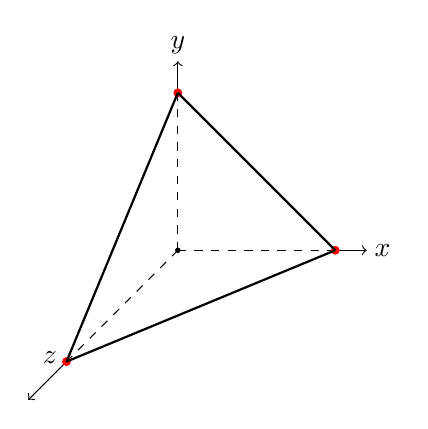
\begin{tikzpicture}[scale=2]
 	\draw[->] (1,0)  -- (1.2,0);
 	\draw[->]  (0,1)  -- (0,1.2);
 	\draw[->]  (-0.7071   ,-0.7071  )  -- (-0.95  ,-0.95 );
 	
 	 	\draw[color=black,dashed] (0,0)  -- (1,0);
 	\draw[color=black,dashed]  (0,0)  -- (0,1);
 	\draw[color=black,dashed]  (0,0)  -- (-0.7071   ,-0.7071  );
 	
 	
 	\fill  (0:0)  circle(0.5pt);
 	
 	\node (P)  at (0:1.3) {$x$} ;
 	\node (P)  at (90: 1.3) {$y$} ;
 		\node (P)  at (220: 1.06) {$z$} ;
 	
 	%% 顶点
 	\fill[color=red]  (0,1)  circle(0.8pt);
 	\fill[color=red]  ( 1,  0)  circle(0.8pt);
 	\fill[color=red]  (-0.7071 ,  -0.7071 )    circle(0.8pt);	
 	
 	
 	\draw[color=black,thick] (0,1) -- ( 1,  0) ; 
 	\draw[color=black,thick] (0,1)  -- (-0.7071 ,  -0.7071 ) ;
 	\draw[color=black,thick] (-0.7071 ,  -0.7071 )    -- ( 1,  0)  ;
 	
 	
 	% 	\node (P)  at (45:0.31) {$A$} ;
 	% 	\node (P)  at (7: 3.45) {$B$} ;
 	% 	\node (P)  at (85:1.03) {$C$} ;

 	\end{tikzpicture}
 		\caption{
 		An intuitive  sketch map 
 	concerning the reformulation  from model (\ref{optmodelori})  to 
 	(\ref{optmodel})  for the case of $n=3$:
 transforming  the regular triangle  from   2D    to  3D  space.
 }
	
 	\label{simplextrans}
 \end{figure}
 
 
 
 
 For   simplicity,  in the later  analysis, denote  
% $ f (\mathbf u) = \sum_{i=1}^{n}  u_{i}^{m} $,  
% $ g_{1}(\mathbf u) =  \mathbf u^{\mathrm T}\mathbf u -1 = 0 $,  
% %  \sum_{i=1}^{n} u_{i}^{2} -1=
% $ g_{2}(\mathbf u) = \mathbf u^{\mathrm T}\mathbf 1_{n} = 0 $.  
\begin{align}
\notag
 & f (\mathbf u) = \sum_{i=1}^{n}  u_{i}^{m}, \\ 
&\nonumber   g_{1}(\mathbf u) =  \mathbf u^{\mathrm T}\mathbf u -1 = 0,  \\
&\nonumber  g_{2}(\mathbf u) = \mathbf u^{\mathrm T}\mathbf 1_{n}-0 = 0 .  
 \end{align}

 
 The  reformulated  model  can  be 
 understood as    a  transformation   that  transfers    the  original model  in $n-1$-dimensional  space  into 
 the $n$-dimensional one  for  analysis. 
And  the  new  constraint  
 $  \mathbf   u^{\mathrm T}   \mathbf   1_{n} =0 $
 is  naturally  related  to   Property  \ref{regularproperty}.
 	An intuitive  sketch map 
 for the case of $n=3$  is  plotted  in  Fig~\ref{simplextrans}.
 
 It should be emphasized that 
 there exists an one-to-one  correspondence relationship 
 between 
 the solutions of 
 (\ref{optmodelori})  and
 those of 
  (\ref{optmodel}).
 When 
 $ \mathbf v$ is a feasible solution of  (\ref{optmodelori}), 
 the corresponding $\mathbf u$ calculated by 
 (\ref{udenote}) 
 will also be a solution of (\ref{optmodel}), and vice verse. 
 Compared to the original  model (\ref{optmodelori}), 
   (\ref{optmodel}) 
   could be 
   with the  following advantage:
   the objective function $f (\mathbf u)$  is 
   separable regarding to the $n$ variables  $u_{i}$, 
  which will be beneficial  to  analyzing 
  the structure 
  for eigenpairs, and this  will be discussed in the   next  two  sections. 
 
%  is  
% transformed into  checking  the locally maximized solutions  of a  reformulated  model.
 Then, in the  following Section  \ref{station} and \ref{locallymaximized},
 the structure for all  the  stationary  and  locally optimal  solutions of 
 the newly reformulated model 
 is investigated  to  sequentially proceed the analysis.
%  \subsection{New Criterion  for  robustness analysis}\label{NewCriterion}
%  
%  
%  
%%  Combining  the  new  reformulated  model   as  stated  in 
%%  the  following  core  is  to  analyze the   structure  of  the  solutions of  and  its  
%%  and  the  details  are   as  follows.
%  
%  
%  Note  that  in  the  related works \cite{RobustEigen,teneigenstructure},
%  the  robustness of  an  eigenpair  is  generally  checked  by the  spectral  radius of the Jacobian  matirx as  defined  in 
%  Subsection   \ref{robustsection}.
% However,  directly  calculating the Jacobian matrix  and  
%  determining the spectral radius  
%  is generally a difficult  task. 
%  For example, 
% in the  previous work \cite{teneigenstructure}, 
% only the case of $n=3$ can be analyzed, while
% it is a little complicated for higher-dimensional  case analysis. 
%
%
%  In this part,  we  would  like  to  provide  an  auxiliary   criterion   for  robustness  checking,  which  then  is  transformed  into  
%analyzing  the  second-order  necessary  condition  of the  optimization model. 
%  	It  can  be  observed   by   comparing    (\ref{Jacobianmatirx})  with   (\ref{hessian_matrix})  
%  that  both  of  them   contain   a  term  $\mathcal{S}  \mathbf{v}^{m-2}$,  and  
%  by  further   investigating  their  relationship,  the  following    lemma  can  be  built:     
%  	\begin{lemma}\label{RobustLocal}
%  	Given  an  eigenpair   
%  	$(\lambda ,\mathbf v )$  of   a  tensor $\mathcal S   \in    T^{m}(\mathbb R^{n}) $, 
%  	if  the eigenpair  is   locally  maximized    solution  of  model (\ref{opti_ori}), 
%  it must be 	a  robust  eigenpair.
%  \end{lemma}
%  \begin{proof}
%  	First,  
%  	$ 	\mathbf {K} $   in  (\ref{Mhess})  is  rewritten  as  the  following  form:
%  	\begin{align}
%  	\mathbf {K}
%  	&   	  	\nonumber 
%  	 =  \mathbf  P_{\mathbf  v}^{\bot} \mathbf H (\mathbf v) 
%  	\mathbf  P_{\mathbf  v}^{\bot} 
%  	\\  	\nonumber 
%  	&=
%  	(\mathbf  I_{n-1}  - 
%  	\mathbf v\mathbf  v^{\mathrm T} )
%  	[ (m-1)\mathcal S \mathbf v^{m-2} - \lambda \mathbf I_{n-1}]
%  	(\mathbf  I_{n-1}  - 
%  	\mathbf v  \mathbf v^{\mathrm T} )
% 	\\  	\nonumber 
%  	&=
%  	(\mathbf  I_{n-1}  - 
%  	\mathbf v\mathbf v^{\mathrm T} )
%  	[
%  	(m-1)\mathcal S \mathbf v^{m-2} 
%  	-
%  	\lambda \mathbf I_{n-1}
%  	-
%  	(m-2)\mathbf v\mathbf v^{\mathrm T}  
%  	]
%   	\\  	\nonumber 	
%  	&=
%  	(m-1)\mathcal S \mathbf v^{m-2} 
%  	-
%  	\lambda \mathbf I_{n-1}
%  	-
%  	(m-2)\mathbf v\mathbf v^{\mathrm T}  
%  	-
%  		(m-1)\mathcal S \mathbf v^{m-2}  	\mathbf v\mathbf v^{\mathrm T}
%  		+
%  			\lambda	\mathbf v\mathbf v^{\mathrm T}
%  			+
%  			(m-2)	\mathbf v\mathbf v^{\mathrm T}
%  		 	\\    	 	\nonumber 
%  			&
%  			=
%  			(m-1)\mathcal S \mathbf v^{m-2} 
%  			-
%  			\lambda \mathbf I_{n-1}
%  			-
%  			(m-1)\lambda \mathbf v \mathbf v^{\mathrm T}
%  			+
%  			\lambda	\mathbf v\mathbf v^{\mathrm T}  ,	
%  			\\    	 	\nonumber 
%  			&
%  			=
%  			(m-1)
%  			( \mathcal S \mathbf v^{m-2} 
%  			-
%  			\lambda \mathbf v \mathbf v^{\mathrm T}
%  			)
%  			-
%  			\lambda 
%  			(\mathbf I_{n-1}
%  			-
%  			\lambda	\mathbf v\mathbf v^{\mathrm T}
%  			)  ,	
%  	\end{align}
%  	where in the second to last equation, we utilize 
%  	$ \mathcal S \mathbf v^{m-2}  	\mathbf v 
%  	= \mathcal S \mathbf v^{m-1}  	
%  	=
%  	\lambda		\mathbf v$.
%  	
%  	By   comparing  with   (\ref{Jacobianmatirx}), it  holds  that  	
%  	\begin{align}
%  	\lambda	\mathbf J =   	{\mathbf K }
%  	+\lambda  (\mathbf  I_{n-1}  - 
%  	\mathbf v \mathbf v^{\mathrm T} ) .
%  	\end{align}
%  	
%  	Note  that  
%  	$  \mathbf  I_{n-1}  - 
%  	\mathbf v  \mathbf v^{\mathrm T}
%  	$ 
%  	is  a  projection  matrix  with  rank  $n-2$, and  its  eigenvalues are given by 
%  	$ 1, 1,   \dots,  1,  0    $,  where the  number  of  the eigenvalue  of  $ 1 $  is  $ n-2 $.  
%  	
%  	%		Assume that 
%  	%		the eigenvalues of  $\mathbf M$
%  	%		is sorted  as 
%  	%		$ \sigma_{1}   \le   \sigma_{2}  \le    \dots  \le \sigma_{n-1} \le \sigma_{n} = \sigma_{max}$.
%  	According  to  the  Weyl  theorem \ref{weyltheo}, 
%  	we can  have  that 
%  	\begin{align}\label{lmdrelation}
%  	\lambda	 
%  	\sigma_{max}  (\mathbf J ) 	
%  	\le    	
%  	\sigma_{max}  (\mathbf K )
%  	+		\lambda    	.
%  	\end{align}
%  	
%  	If  	
%  	$(\lambda ,\mathbf v )$  is    a   locally  maximized    solution  of  model (\ref{opti_ori}), 
%  	its  corresponding   matrix 
% $  	\mathbf K  $ 
% will be  a  negative  definite one,  indicating 
%  	$   	\sigma_{max}  (\mathbf  K)  <  0 $.
%  	By  combining  (\ref{lmdrelation}), it can be  concluded that 
%  	\begin{align}\label{lmdrelationmax}
%\lambda	 
%\sigma_{max}  (\mathbf J ) 	
%\le    	
%\sigma_{max}  (\mathbf K )
%+		\lambda    	
%< 
%\lambda  ,
%\end{align}
%which  indicates that
%  	\begin{align}
%  	\vert \sigma_{max}  (\mathbf J ) 	\vert
%  	< 1.
%  	\end{align}
%  	And  the proof is complete.
%  \end{proof}
%
%
%
%%   is   a  robust  one,  the  maximized  eigenvalue for  the matrix  $\mathbf M$  is  always  less  than  0,  which  means that  it  is  a   matrix.
%%By  Theorem \ref{theosecond_order_necessary} ,  the  corresponding  eigenpair is a  locally  maximized ones.
%%In  this  way,  the  equivalence  between  the  robustness and  local optimality   of  eigenpairs
%%can be  established. 
%%Then, 
%
%\begin{remark}\label{necessaryonly}
%%	The  motivation of  developing  the above lemma 
%%	is  due to the difficulty of explicitly  expressing  the result of the Jacobian matrix  	$ \mathbf{J}(\mathbf{v}) $, 
%%	and of  determining its spectral radius let alone. 
%%	For example,  the researchers  only analyzed  the  case of $n=3$, while
%%	it is a little complicated for higher-dimensional  case analysis. 
%	The  above lemma provides  a   sufficient   condition for the robustness identification. 
%%	In  the  later proof, we will  utilize the above conclusion to  analyze the local optimality of eigenpairs. 
%	It should be emphasized that the 
%	local optimality  is still not a  necessary  condition 
%	for the  robust eigenpairs  according to the above lemma. 
%	In  other words, 
%	if  an  eigenpair is a  robust one, it 
%	may not always be a locally maximized one. 
%	This can be observed from 
%	(\ref{lmdrelationmax}).
%	If  the eigenpair  is robust, we cannot  obtain that  the maximized eigenvalue for 
%	$\mathbf M$ is definitely negative. 
%	
%
%\end{remark}


%In this remark, we  briefly 
%illustrate the advantage of using second-order necessary condition as mentioned above.
%As can be observed from the calculation of 
%$ \mathbf{J}(\mathbf{v})$  in  (\ref{Jacobianmatirx}),
%the criterion  by  checking the spectral radius   cannot deal with the case where eigenvalue is equal to 0.
%For example, when $n=3, m=3,$, previous paper \cite{teneigenstructure} has shown that  the tensor has  three  eigenpairs  whose eigenvalues are 0. 
%Therefore, 
%using (11) cannot deal with  the  robustness  of these eigenvalues. 
%See Table 1 in  \cite{teneigenstructure}  for more  similar  cases. 
%In contrast, the new criterion 
%can avoid this problem, where 
%$ 	\mathbf {M} $ of each solution
%can be well defined. 
  
%  In this part,  we would like to provide a new   criterion  to  identify  whether an  given  eigenpair  is  robust or not.
  
  % \subsection{Statistical interpretation for  regular  simplex  tensor\ref{Theorem_optimal}}\label{Simpleillustration}

 
% \section{Structure of  solutions of  (\ref{optmodel})}%\label{station}
%By  Lemma  \ref{RobustLocal},
%if  the  corresponding  second-order  matrix $\mathbf   K$  of  an  eigenpair  is  
%negative  definite, 
%this eigenpair  must be a robust.
%In this way,  
%we can  resort  to  checking the  second-order   necessary  condition  of  the  constrained  model  to 
%analyze the robustness of  these vectors in the frame. 
%% In the  following,  we  will   adopt  such a   way  to  proceed  our  proof.
%Due to the equivalence of    (\ref{optmodelori})  and (\ref{optmodel}), 
% in  the  following  two sections,   we  will  mainly  focus  on  the  reformulated  model   (\ref{optmodel})  and   analyze  its   stationary  and  locally  maxmized  solutions  by    sequentially  
% checking the  first-order  KKT   and  second-order   necessary  condition, 
% which  
% corresponds to the  two key  steps as  explained in the proof outline,  respectively.
 

 \section{Structure  of  all  stationary points of  (\ref{optmodel})}\label{station}
The Lagrangian function  of the  reformulated  constrained  model in  (\ref{optmodel})    is 
defined as:
\begin{equation}\label{Lagrangianfunctionnew}
L(\mathbf u, \alpha, \beta)=
\frac{1}{m}
\sum\limits_{i=1}^{n}  u_{i}^{m}						%\sum_{i=1}^{n} u_{i}^{3}
+
\frac{\alpha}{2}
(1- \mathbf   u^{\mathrm T}   \mathbf   u  )
+
\beta (0- \mathbf   u^{\mathrm T}   \mathbf   1_{n}),
\end{equation}
where $ \alpha,\beta$ are  the  corresponding   Lagrangian   multipliers of  the two  constraints.

To  obtain all the stationary points, one can  check  the first-order  necessary   condition
(also known as Karush-Kuhn-Tucker (KKT) condition)
of model  (\ref{optmodel}).
The gradient of
$  L(\mathbf u, \alpha, \beta) $    with  respect  to  
$ \mathbf u $   follows: 
\begin{equation}\label{gradient}
\triangledown_{\mathbf u}L =
\mathbf u ^{\circledast^{m-1}}
-
\alpha \mathbf u-\beta \mathbf  1_{n} . 
\end{equation}


% To  obtain all the stationary points
 When
$ \triangledown_{\mathbf u}L = \mathbf 0$,  it  holds  that 
\begin{equation}
\notag
\mathbf u ^{\circledast^{m-1}}-\alpha \mathbf u-\beta \mathbf  1_{n} = \mathbf 0 . 
\end{equation}

To   conclude,  the  
stationary points of  (\ref{optmodel})
should  simultaneously 
satisfy 
  the  following  three  equations:  
\begin{align}
\label{KKTgradient}
&\mathbf u ^{\circledast^{m-1}}-\alpha \mathbf u-\beta \mathbf  1_{n} = \mathbf 0 . 
\\
\label{KKTcon1}
&\mathbf   u^{\mathrm T}   \mathbf   u =1 .
\\
\label{KKTcon2}
&\mathbf   u^{\mathrm T}   \mathbf   1_{n} =0.
\end{align}

By multiplying  $\mathbf   u^{\mathrm T}$ on  both sides of (\ref{KKTgradient}) and utilizing  (\ref{KKTcon1})  and
(\ref{KKTcon2}), 
we can  obtain  that 
\begin{align}\label{alphares}
\alpha 
=
\sum\limits_{i=1}^{n}  u_{i}^{m}
=
f(\mathbf u).	
\end{align}

Similarly, by multiplying  $  \mathbf   1_{n}^{\mathrm T}$ on  both sides of (\ref{KKTgradient}) and utilizing  (\ref{KKTcon1})  and
(\ref{KKTcon2}), 
 we can  obtain  that 
\begin{align}\label{beatres}
\beta 
=
\frac 1 n  \sum\limits_{i=1}^{n}  u_{i}^{m-1}.	
\end{align} 


\begin{figure*}[t]
	\centering
	\begin{subfigure}[htbp!]{0.39\textwidth}
		\includegraphics[width=1\textwidth]{pic/odd.eps}
		\subcaption{}
		\label{odd}
	\end{subfigure}
	\begin{subfigure}[htbp!]{0.39\textwidth}
		\includegraphics[width=1\textwidth]{pic/even.eps}
		\subcaption{}
		\label{even}
	\end{subfigure}
	\caption{
		\quad 
		The  sketch figures   for the curve  of   the  function   $  f(x) = x^{m-1} -\alpha x - \beta$ for odd and even case:  a)   odd  $m$  case: $m=3, \alpha=1, \beta =2$;   b)   even   $m$  case: 
$m=4, \alpha=7, \beta =4$.	}
	\label{curveplot}
\end{figure*}


\begin{remark}
	Note that both 
	$\alpha$ and $\beta$ 
	are the function of $\mathbf u$. 
	For simplicity, we omit the variable  $\mathbf u$ in the notations.
We  discuss the sign of $\alpha $ and  $\beta $  for  different orders $m$. 
When  $m$  is odd, 
since $\alpha(-\mathbf u) = -\alpha(\mathbf u) $,  we can always select  the value where $\alpha >0$. 
For $\beta$ which  is the summation of  $n$ non-negative  terms,  it  holds that  $\beta \ge 0$. 
However, considering the  constraint  in  (\ref{KKTcon1})  and
(\ref{KKTcon2}), all $n$ terms $u_{i}$ cannot be equal to 0 simultaneously.
Therefore, we can  finally  conclude that 
 $\beta > 0$. 
A similar  analysis can be proceeded   for the even $m$  case,  and it  holds that  $\alpha >0$  and  $\beta \ge 0$.
\end{remark}

Then,  as can be  observed  from (\ref{KKTgradient}),  each $u_{i}$   can  be  one of  the roots  of  $(m-1)$-order polynomial 
$ u_{i}^{m-1} -\alpha u_{i} - \beta =0  $.
Note that  in  this  paper,  we  only  discussed  the  real  solutions, consistent with the previous work \cite{teneigenstructure}.
By plotting  the  function  curves 
with  the  form  of 
 $  f(x) = x^{m-1} -\alpha x - \beta$
   for  odd  and  even  two  cases,  
it can be observed  from  Fig 	\ref{curveplot} that 
when $m$ is odd,  there are  at most  two  real  roots  for  $ u_{i}^{m-1} -\alpha u_{i} - \beta =0  $, 
while  $m$ is even,  the number  turns  to be three ones. 
Therefore, throughout  the  following  contents,  we  will  separately discuss  the odd and  even   $m$ cases.
Note that  such  an  observation  and  classification  rule is  consistent with the  discussion  presented in 
the previous work \cite{teneigenstructure}.
The  differences  lie  in  that 
\cite{teneigenstructure}  focuses   on the original model (\ref{optmodelori}), while  
this paper analyzes the  reformulated one (\ref{optmodel}).
%This  also further  confirms  the  equivalence between  the  two  models.
%A  detailed comparison can refer  to Table \ref{tableforcomparison}.

And the  following  Lemma  concludes
the structure and number  of all  the  stationary  solutions for model (\ref{optmodel}):
\begin{lemma}\label{Theorem_structureofall}
%	Let  $ \mathbb  A $   be  the  set  of  any   $ k$  $(1 \le  k  \le n-1)$  integers     selected  from   the  set    of   $n$    integers  $ \{  1,2,\dots, n \} $. 
	
	i):
	when  $m$  is  odd, 
	all  the  stationary   points  of    model (\ref{optmodel}), 
	$	\mathbf   u =  
	[u_1,u_2,\dots, u_{n}]^{\mathrm T} \in  \mathbb {R}^{n \times 1}  $, 
	are  with   the  structure as  follows:
%	\begin{equation}\label{u_classify}
%	\mathbf   u =   
%	%	[u_1,u_2,\dots, u_{n}]^{\mathrm T}=
%	[u_{i}]_{i=1}^{n}
%	=
%	\begin{cases}
%	a ,  \quad  \quad    i   \in  \mathbb A      \\
%	b ,    \quad  \quad           i    \notin   \mathbb A  
%	\end{cases}  ,
%	\end{equation}
		\begin{equation}\label{u_classifyodd}
\mathbf u
=
\mathbf P
[
a \mathbf 1_{k}^{\mathrm T},
b \mathbf 1_{n-k}^{\mathrm T}
]^{\mathrm T}, 
\end{equation}
	where  
	$ a=   \sqrt{	\frac{n-k} {k n}		} >0 $  and  
	$  b=-  \sqrt{	\frac{k} {(n-k) n}	}   <0 $ vary with $k$, 
	where $1 \le  k  \le \lceil n/2  \rceil $, ($\lceil n/2  \rceil$ denotes the 
	integrate that is no larger than $ n/2 $)
	and
	$\mathbf P \in  \mathbb R^{n \times n} $
	is  a 
	permutation matirx. 
	
			ii):
		when  $m$  is  even, 
		all  the  stationary   points  of    model (\ref{optmodel}), 
		$	\mathbf   u =  
		[u_1,u_2,\dots, u_{n}]^{\mathrm T} \in  \mathbb {R}^{n \times 1}  $, 
		are  with   the  structure as  follows:
		\begin{equation}\label{u_classifyeven1}
		\mathbf u
		=
		\mathbf P
		[
		a \mathbf 1_{k}^{\mathrm T},
		b \mathbf 1_{n-k}^{\mathrm T}
		]^{\mathrm T}
		\end{equation}
		or 
		\begin{equation}\label{u_classifyeven2}
		\mathbf u
		=
			\mathbf P
			[
		c \mathbf 1_{p}^{\mathrm T},
		d \mathbf 1_{q}^{\mathrm T},
		e \mathbf 1_{s}^{\mathrm T}
		]^{\mathrm T}
		\end{equation}
			where  
		$ a=   \sqrt{	\frac{n-k} {k n}		} >0 $  and  
		$  b=-  \sqrt{	\frac{k} {(n-k) n}	}   <0 $ vary with $k$, 
			where $1 \le  k  \le \lceil n/2  \rceil$,  
		and
		$\mathbf P \in  \mathbb R^{n \times n}$
		is  a 
		permutation matirx;
			where $1 \le  p,q,s  \le n-1$ and    $p+q+s=n$.
		Note that there is no   explicit expression for the variables  $c,d,e$
		in (\ref{u_classifyeven2}).
		
			iii): when  $m \ge 3 $ is  odd and $n \ge 3$,  the number of all the stationary points of  model (\ref{optmodel}) is equal to  $	K_{m,n} = 2^{n-1}-1$.
			
		iv): when  $m \ge 3 $ is  even  and $n \ge 3$ ,  the number of all the stationary points of  model (\ref{optmodel}) is equal to 
		\begin{align}
		K_{m,n}=
	\begin{cases}
 \frac 
{ 3^{ n-1} - 1}
{2}  , \quad   n \ge  3, m\ge 4  \\
6  , \quad \quad \quad  n=3, m\ge 6
	\end{cases}.
		\end{align}
		
\end{lemma}


\begin{proof}
%	In term of (i), 
	Equivalently,  for (\ref{KKTgradient}), there   are   $n$  equations  with  the  form of 
\begin{equation}\label{uim1alpha} 
u_{i}^{m-1} -\alpha u_{i} - \beta =0  \quad  (i=1,2, \dots, n).
\end{equation}

%\begin{equation} 
%u_{j}^{m-1}  -\alpha u_{j} - ( u_{i}^{m-1} -\alpha u_{i}  )  =0  \quad  (j=2, 3,\dots, n).
%\end{equation}
%Subtracting  the  last  $n-1$  ones  from    the  first one and  with  some  rearrangement, we  obtain  
%$n-1$  equations  that  follow:
%\begin{equation}\label{n1equations}
%\left\{\begin{array}{c}
%(u_{1}-u_{2})	(u_{1}^{m-2} + u_{1}^{m-3} u_{2} + \dots + u_{2}^{m-2} -\alpha)=0 \\
%(u_{1}-u_{3})	(u_{1}^{m-2} + u_{1}^{m-3} u_{3} + \dots + u_{3}^{m-2} -\alpha)=0  \\
%\vdots \\
%(u_{1}-u_{n})	(u_{1}^{m-2} + u_{1}^{m-3} u_{n} + \dots + u_{n}^{m-2} -\alpha)=0 
%\end{array}\right.
%\end{equation}

In term of (i), 
when $m$ is  odd,  there  are  two  real  roots for 
(\ref{uim1alpha}), 
  denoted by $a,b$ for  simplicity. 
It can be  checked that 
all  $n$ variable 
$u_{i}$ cannot  simultaneously 
be  $a$  or  $b$. 
Otherwise, we  will 
 derive    $ u_{1} =u_{2} = \dots = u_{n}$, which  is contradicted   with  the  constraints  in  (\ref{optmodel}).


Therefore, there  are  at  most  $n-1$ 
variable  
$u_{i}$ 
can be the  same  one. 
For  example, 
assume  that  the  first  $k$ ($ 1 \le  k  \le  n-1 $)  
variables  are the  same, 
and 
the last   $n-k$ fractions  are the other one. 
The  form of the  solution  is  given by 
\begin{align}\label{ab_struc}
& u_{1}=u_{2} \cdots=u_{k}  =a  ,  
&u_{k+1}=u_{k+2}  \cdots=u_{n} =b.  
\end{align}

%\begin{equation}\label{n1equations}
%\left\{\begin{array}{c}
%	u_{1}^{m-2} + u_{1}^{m-3} u_{k+1} + \dots + u_{k+1}^{m-2} -\alpha=0 \\
%	u_{1}^{m-2} + u_{1}^{m-3} u_{k+2} + \dots + u_{k+2}^{m-2} -\alpha=0  \\
%\vdots \\
%	u_{1}^{m-2} + u_{1}^{m-3} u_{n} + \dots + u_{n}^{m-2} -\alpha=0 
%\end{array}\right.
%\end{equation}

%\begin{equation}%\label{n1equations}
%\begin{bmatrix}
%-a   &   -a^{2}      & \dots   &   -a^{m-3} &  \alpha -a^{m-2}  \\
%-1   &   0    &    \dots   &  0 &  0  \\
%0  &  -1  &    \dots   &  0 &  0  \\
%\vdots  & \vdots  & \ddots  & \vdots & \vdots  \\
%0  &  0    & \dots   &   -1 & 0  \\
%\end{bmatrix}
%\end{equation}



%\begin{align}\label{ab_struc}
%& u_{1}=u_{2} \cdots=u_{k}  =a  ,  
%\\
%&
%u_{1}^{m-2} + u_{1}^{m-3} u_{j} + \dots + u_{j}^{m-2} -\alpha \\&= 
%u_{1}^{m-2} + u_{1}^{m-3} u_{k} + \dots + u_{k}^{m-2} -\alpha  
%\end{align}
%For  simplicity,   we  denote  that 
Considering  the  two constraints  in  (\ref{optmodel}), we  have  that 
\begin{equation}\label{ab_expreess}
\begin{cases}
k a^{2}+(n-k) b^{2}=1 \\
k a+(n-k) b=0
\end{cases}. 
\end{equation}
Then, it can be derived that 
\begin{equation}\label{ab_solu}
\begin{cases}
a=   \sqrt{	\frac{n-k} {k n}		} \\
b=-  \sqrt{	\frac{k} {(n-k) n}	}  
\end{cases},
\quad  or  \quad 
\begin{cases}
a=   - \sqrt{	\frac{n-k} {k n}		} \\
b=  \sqrt{	\frac{k} {(n-k) n}	}  
\end{cases},
\end{equation}
where  
$ a, b  $ vary with $k$. %, and  for simplicity, we omit the subscript $k$ in both $ a, b$.
Furthermore, note  that   because  
 $ f ( -\mathbf  u ) = -  f (\mathbf  u) $  when  $m$ is odd,
we thus can   only reserve   the former  one solution   in (\ref{ab_solu})  where  $ a>0$ .
Then,  the  structure of  all   solutions
can be  denoted  by 
permuting the  indices  of  $i$  by  a  permutation matrix $\mathbf P$, which then  
can be  expressed as  the form in 
(\ref{u_classifyodd}).

In term of (ii), 
when $m$ is  even, 
there  are  at  most  three  real  roots for 
(\ref{uim1alpha}).
Similarly,  all $n$  variables  cannot be the same one, indicating  that there  are  at  least  two  different  values  concerning  the components of $\mathbf  u$.
Then, the  analysis can be similarly  proceeded  as  that  in (i)
and  the structure  of  
the solution will be  given by 
(\ref{u_classifyeven1})
and 
(\ref{u_classifyeven2}).
Note that 
for  (\ref{u_classifyeven1}), 
the value of $a$ and $b$ can be the same as the odd $m$ cases.
While 
for 
(\ref{u_classifyeven2}), 
since we have  three  unknown  variables $c,d,e$
but only  two  constraints, we cannot 
obtain the  explicit  expression  for $c,d,e$.








In term of (iii),   
since  each $u_{i}$ can be  selected  as  one  of  two real  roots,
the total combination numbers   are  given by 
$2^{n}$.
First,  
the  case that  
all $n$   
$u_{i}$ are the same one should be  excluded, as analyzed before. 
In addition, 
in the left 
$2^{n}-2$
combinations, 
it contains  repeated  same solutions, for  example, 
$ [
a \mathbf 1_{k}^{\mathrm T},
b \mathbf 1_{n-k}^{\mathrm T}
]^{\mathrm T} $
and 
$ [
b \mathbf 1_{k}^{\mathrm T},
a \mathbf 1_{n-k}^{\mathrm T}
]^{\mathrm T} $
can be treated as the same one solution. 
This is the reason that we constraint $1 \le  k  \le \lceil n/2  \rceil$,
since the solutions
where $\lceil n/2  \rceil  \le  k  \le  n-1$
can be considered as the same one. %with those 
Therefore, the   total  number of 
feasible solutions 
is  given by 
$
\frac{2^{n}-2}{2}
=
2^{n-1}-1$.


In term of (iv),   for the  even $m$  case,  
it can be analyzed in a  similar way to that in (iii).
Since  one special 
case 	 of 		$n = 3, m = 4$ 
is excluded out of the scope,  as 
explained in Remark \ref{RemarkScope},
the number of all  solutions 
is separately discussed    from two different cases. 
In the first case where 
$ n=3, m\ge 6 $, 
it is easy to conclude that 
there are totally 6  solutions, 
counting three ones for both 
(\ref{u_classifyeven1})
and 
(\ref{u_classifyeven2}).
In the second  case where 
$  n \ge  3, m\ge 4 $, 
similar to the analysis for the odd $m$ case, 
 the  number  of 
all stationary  solutions 
is   
eventually 
given by 
$ \frac 
{ 3^{ n-1} - 1}
{2}  $.
And the proof is complete.
\end{proof}

\begin{remark}
	Note that in 
	(\ref{u_classifyeven1})
	and 
	(\ref{u_classifyeven2}),
	we use five notations  from 
	$a$ to $e$ to distinguish 
	the  two  different   structures   of  the solutions for the even $m$ cases. 
	We wish that  such a  distinction 
	will not cause ambiguity 
	concerning the fact that there are at most three different  real roots for 
		$  u_{i}^{m-1} -\alpha u_{i} - \beta =0  \quad  (i=1,2, \dots, n) $
		when $m$ is even. 
\end{remark}

After  having  investigated the structure of all  stationary  solutions, 
the  following lemma can be  established to 
reveal  the  relationship 
between the vector in the frame (which is the generators of the corresponding regular simplex tensor) and 
all stationary solutions: 
\begin{lemma}\label{vectorregularsimplexframe}
	The  vectors   in the regular simplex  frame, i.e., 
	 $ \mathbf{w}_{1}, \ldots, \mathbf{w}_{n}$,
	 correspond  to 
	 eigenpairs when $k=1$  in both   
	 (\ref{u_classifyodd})  and (\ref{u_classifyeven1}). 
	\end{lemma} 


\begin{proof}	
	Concerning  the   vectors   in the regular simplex  frame
 $
 \mathbf W =
 [
 \mathbf{w}_{1}, \ldots, \mathbf{w}_{n}
 ] \in
  \mathbb{R}^{(n-1) \times  n}$, 
  it holds that 
 $ \mathbf{w}_{i}^{\mathrm T} \mathbf{w}_{i} =1, 
  \mathbf{w}_{i}^{\mathrm T} \mathbf{w}_{j} = \alpha = -\frac{1}{n-1} $
  for 
  $ i \neq j$. 
  It can be calculated that  when 
  $ \mathbf v = \mathbf w_{j}$,
  it holds that 
 \begin{align}\label{udenotealpha}
\mathbf   u 
& 
\nonumber =
\sqrt {
	\frac  {n-1}{ n}
}   
{\mathbf W}^{\mathrm T}  {\mathbf w_{j}}  
= 
[u_1,u_2,\dots, u_{n}]^{\mathrm T} 
\\
&=
\sqrt {
	\frac  {n-1}{ n}
} 
[\alpha,  \dots,   \alpha, 
\underbrace{ 1 }_{j}, \alpha,  \dots,  \alpha ]^{\mathrm T} 
\in  \mathbb {R}^{n \times 1} ,
\end{align} 
It can be checked that 
$\mathbf u$ with the above form satisfies the two constraints  in (\ref{optmodel}).
Clearly,  
when $ \mathbf v = \mathbf w_{j}$,
$\mathbf u$  in   (\ref{udenotealpha}) 
correspond to the solutions  of   $k=1$ of 
(\ref{u_classifyodd})  and (\ref{u_classifyeven1}), and 
it holds for both odd  and even cases.
By  the equivalence  between  (\ref{optmodelori}) and  (\ref{optmodel}),
all  the 	  vectors   in the regular simplex  frame, i.e., 
$ \mathbf{w}_{1}, \ldots, \mathbf{w}_{n}$,
correspond  to 
$n$
eigenpairs  of the regular simplex  tensor. 
\end{proof} 
%based on the above analysis, we can also enumerate the number of all the stationary points of 
%model (\ref{optmodel}). 
%There are $ \left(\begin{array}{c}
%n-1 \\
%n-k
%\end{array}\right)
%1^{k}
%(m-2)^{n-k-1}
%$ 
%solutions when any random $n-k$ equations of (\ref{u_n}) are chosen to be true. Since $ 1 \le  k  \le  n-1 $,  the number of solutions of (\ref{optmodel}) in total, denoted $  K_{m,n}$,  is equal to  
%\begin{align}\label{numofpoint}
%K_{m,n}
%\nonumber 
%&= 
%\sum_{k=1}^{n-1} \left(\begin{array}{c}
%n-1 \\
%n-k
%\end{array}\right)
%1^{k}
%(m-2)^{n-k-1}
%\\  \nonumber   & =
%\sum_{k=1}^{n-1} \left(\begin{array}{c}
%n-1 \\
%k-1
%\end{array}\right)
%(m-2)^{n-k-1}
%\\ \nonumber   & =
%\sum_{k=0}^{n-2} \left(\begin{array}{c}
%n-1 \\
%j
%\end{array}\right)
%(m-2)^{n-j-2}
%\\   \nonumber  & =
%\sum_{k=0}^{n-1} \left(\begin{array}{c}
%n-1 \\
%j
%\end{array}\right)
%(m-2)^{n-j-2}
%\\   \nonumber 
%& \quad -
%  \left(\begin{array}{c}
% n-1 \\
% n-1
% \end{array}\right)
% (m-2)^{n-(n-1)-2}
%\\    
%&= 
%\frac 
%{ (m-1)^{ n-1} - 1}
%{m-2} .
%\end{align}
%%$\blacksquare$




%\begin{align}\label{numofpoint}
%K_{m,n} 
%=
% 2^{ n-1} - 1
%\end{align}

%\begin{align}\label{numofpoint}
%K_{m,n} 
%=
%
%\end{align}


%\subsection{The number  of  real  and  complex  eigenpairs}\label{seccond}
%
%\begin{theorem} \cite{upperbound}
%	If a tensor $\mathcal S   \in    T^{m}(\mathbb R^{n})  $  has finitely many equivalence classes of  eigenpairs over 
%	$ \mathbb  C$,   then their number,
%	counted with multiplicity,     is   bounded  by  
%	\begin{equation}\label{at_most}
%	M(m,n)=
%	\frac {(m-1)^{n}-1}  {m-2}.
%	\end{equation}
%\end{theorem}


%Note that    by   analyzing  the  first-order   gradient  information  of  (\ref{Lagrangianfunctionnew}), we  have   deduced  the   structure  of  all   stationary   points. 
%Besides, (\ref{numofpoint}) also indicates that the total number of all the stationary points is no less than the number of vertices of the simplex  $n$ ($n \ge 3$). 
%In  optimization  theory,   not  all  stationary  points  correspond  to  the  locally  optimal    ones. 
%Actually, some   stationary points  can  be categorized as   saddle points.
%To  recognize   the  local   maximum,   we  further  consider  the  second-order   derivation  information  of  (\ref{Lagrangianfunctionnew}), and the details  are  follows.


%; 
%2) Among  $K_{n}$  solutions,  the solution for    the  first    $k-1$   are 
%true  and  for  the  last  $n-k$ are  true     are  indeed  equivalent.  $\blacksquare$
%	range   from 1 to 
%	$\lfloor      n/2  \rfloor$, since  for  $k \in  [ \lfloor      n/2  \rfloor+1, n-1]$, 
%	$ \mathbf u$ is     in  the  opposite directions compared to those for  
%	 $k \in  [ 1,  \lfloor      n/2  \rfloor]$. 
	

%Note  that  given  a   certain  $k$,   the  permutation  of  $  u_{1}, u_{2}, \dots, u_{k} $   is  trivial,  since  the  model (\ref{optmodel})  is  symmetric  concerning such  a  permutation.
%For  convenience  in the  later  analysis, which will be  seen from (\ref{publock})  $\sim$ (\ref{Hblock}), we  always   intellectually   rearrange  the  elements  of  $\mathbf u$  to  be  two  partitioned   bolcks.  


%$u_{k+1}=u_{k+2}=\cdots=u_{n}$
%\begin{equation}\label{u_block}
%\mathbf u=( 
%\underbrace{  a, a, \cdots, a}_{k}, 
%\underbrace{b, b, \cdots, b}_{n-k}
%)^{\mathrm  T}
%\end{equation}



%\begin{table*}[t]
%	\normalsize
%	\centering
%	\caption{\\ Concerning the  model (\ref{optmodel}), the intuitive comparison of all  stationary points (denoted $	\mathbf   u$)  and  locally maximized points (denoted $	\mathbf   u^{\ast}$), where $ \mathbb  A $   be  the  set  of  any   $ k$  $(1 \le  k  \le n-1)$  integers     selected  from   the  set    of   $n$    integers  $ \{  1,2,\dots, n \} $, $ i $   be  an    integer     selected  from    $ \{  1,2,\dots, n \} $. }
%	\label{cc1}
%	\renewcommand\arraystretch{1.4}
%	\begin{tabular}{  |c | c | c |   }
%		\hline
%		%\cline{1-3}
%		&  stationary points  &  locally maximized points \\
%		\hline
%	%\cline{1-3}
%Satisfied Condition 	&  First-order  necessary (or KKT)  condition   &  Second-order  necessary  condition  \\
%\hline
%		Structure of solutions 
%		& $	
%		\mathbf   u =   
%		[u_{i}]_{i=1}^{n}
%		=
%		\begin{cases}
%		a ,  \quad  \quad    i   \in  \mathbb A      \\
%		b ,    \quad  \quad           i    \notin   \mathbb A   
%		\end{cases}
%		$
%		& $ \mathbf  u^{\ast} =
%		[b,b,\dots, 
%		b,
%		\underbrace{ a }_{i}, 
%		b, \dots, b]^{\mathrm  T} $   \\
%		\hline
%		Number of solutions 
%		&  $ K_{n}=2^{n-1}-1$ 
%		&  $n $
%		\\
%		\hline
%		Summary 
%		&  Lemma  \ref{Theorem_structureofall}
%		&  Lemma \ref{Theorem_structureoflocal}
%		\\
%		\hline
%	\end{tabular}
%	\label{tableforlemma}
%\end{table*}







%Before  proceeding  our  proof, the following lemma\cite{Numerical} is   useful for  the constrained optimization problem to identify   the  locally  optimal points:
%%\setcounter{theorem}{3}
%\begin{lemma}[\textbf{Second-order necessary condition\cite{Numerical}}]\label{theosecond_order_necessary}
%	Suppose that
%	for any  vector $ \mathbf w \in \mathbb V $,
%	\begin{equation}%\label{second_order}
%	\mathbf w^{\mathrm H}\mathbf H (\mathbf u^{\ast}) \mathbf w  \le 0   % \preceq
%	\end{equation}
%	holds, then
%	$\mathbf u^{\ast}$
%	is a local maximum solution of (\ref{optmodel}).
%	And in this case, the set
%	$\mathbb V $
%	is defined as
%	\begin{equation}\label{vset}
%	\mathbb V=\{
%	\mathbf w \in \mathbb R^{n}
%	\vert   \mathbf A^{\mathrm H} \mathbf w   =\mathbf  0
%	\}=
%	\rm Null [\mathbf A^{\mathrm H} ],
%	\end{equation}
%\end{lemma}
%where  
%
%If a stronger condition, i.e.,
%$ \mathbf w^{\mathrm T}\mathbf H (\mathbf u^{\ast}) \mathbf w  <   0 $,   %\prec
%is satisfied, then,  
%$\mathbf u^{\ast}$
%is a strict  local maximum  solution of (\ref{optmodel}).




%\setcounter{theorem}{0}

 \section{
 %	Proof for Theorem \ref{maintheorem}
 Structure   of  all  locally optimal  points of  (\ref{optmodel})
 }
 \label{locallymaximized}

%\section{Second-order  necessary  condition}\label{seccond}
%\setcounter{theorem}{5}

We have investigated the  structure of all  stationary points of  (\ref{optmodel})  in the above section,
and also shown that 
the vectors in the regular simplex frame 
correspond to 
the solution  of (\ref{optmodel}) when $k=1$  in (\ref{u_classifyodd})  and (\ref{u_classifyeven1}). 
In this section,  we are further interested in identifying  the local optimality of each eigenpair, 
i.e., 
which    are   the  locally  maximized,  minimized or saddle    ones  of (\ref{optmodel})
among    these  solutions.
In other words, we tend to   group 
all these eigenpairs into three classes. 
For this purpose,    it is necessary to   introduce the second-order
derivative information 
of  the  Lagrangian function.      
For  (\ref{Lagrangianfunctionnew}),   the second-order derivation  to    $ \mathbf u $, termed  the Hessian matrix,  is   denoted
\begin{equation}\label{Hessianmatrix}
\triangledown_{\mathbf u\mathbf u}^{2} L
= \mathbf H (\mathbf u)  
=(m-1) diag (\mathbf u ^{\circledast^{m-2}})
-\alpha \mathbf  I_{n}  .
\end{equation}
Similar to 
the  derivation for (\ref{Mhess}),
the 
locally    optimal   solutions of   (\ref{optmodel})
can  be  identified  by
checking the  negative 
definiteness of the  following  matrix:
\begin{equation}\label{Mhess2} 
\mathbf {M} =
(\mathbf  P_{\mathbf  A } ^{\bot})^{\mathrm T}    \mathbf H (\mathbf u)  \mathbf  P_{\mathbf  A }^{\bot}
=
\mathbf  P_{\mathbf  A } ^{\bot}   \mathbf H (\mathbf u)  \mathbf  P_{\mathbf  A }^{\bot}
,
\end{equation} 
where 
$ \mathbf A $
is determined by
the 
two constraints 
$  g_{1}(\mathbf u) $ and  $ g_{2}(\mathbf u) $,
which 
is with the  following form:
\begin{equation}
\label{Aform}
\mathbf A =  [\triangledown  g_{1}(\mathbf u) , \triangledown  g_{2}(\mathbf u) ] =
[\mathbf u, \mathbf 1_{n}]  \in   \mathbb R^{n  \times 2 } .
\end{equation}
And the  detailed  explanation for  the  
derivation of 
(\ref{Mhess2})
are also  presented in  the Appendix part. 

%With this matrix,  
%we than analyze 

%\subsubsection{Odd  $m$  cases } 

Similarly,
we will separately discuss the cases of odd and even order.
Meanwhile, 
as there are three structure as presented 
from  
	(\ref{u_classifyodd})
to
(\ref{u_classifyeven2}),
these   three different cases are 
separately analyzed in the following subsections.
The details are as follows.

 \subsection{Odd  $m$ case}
 
 In this subsection, we first 
 focus on the tensor with  odd  $m$,
 whose solutions 
 are as shown in 
 (\ref{u_classifyodd}). 
\begin{lemma}\label{Theorem_structureoflocal}
	For the case where   $m$ is odd,  concerning  the solutions 
with the form of 
	(\ref{u_classifyodd}):
	i):
	 when  $k=1$ 
	 the solutions  are   the  locally maximized    points  of    model (\ref{optmodel});
	 ii)  when  $2 \le  k \le \lceil n/2  \rceil $, all the other solutions are  the saddle points  model (\ref{optmodel}). 
	
%	Let  $ i $   be  an    integer     selected  from   the  set    of   $n$    integers  $ \{  1,2,\dots, n \} $: 
%	
%	i):
%	All  the  locally maximized    points  of    model (\ref{optmodel}), denoted 
%	$	\mathbf   u^{\ast} =  
%	[u_1,u_2,\dots, u_{n}]^{\mathrm T} \in  \mathbb {R}^{n \times 1}  $, 
%	are  with   the  structure as  follows:
%	\begin{equation}\label{ulocal_classify}
%	\mathbf  u^{\ast} =
%	[b,b,\dots, 
%	b,
%	\underbrace{ a }_{i}, 
%	b, \dots, b]^{\mathrm  T},
%	i = 1,2,\dots, n, 
%	\end{equation}
%	which, clearly,  is  a subset of (\ref{u_classifyodd}) when  $k=1$,  and  
%	all  vectors in the regular  simplex frame 
%	are robust. 
	
%	ii): the number of all  the  locally maximized    points of  model (\ref{optmodel}) is equal to  the number of the vertices of the simplex, $n$.
\end{lemma}

\begin{proof}
%	We first prove (i). 
	Due to the form of $\mathbf  A$ as shown in (\ref{Aform}), 
$ \mathbf  P_{\mathbf  A }^{\bot} $ can be   further  rewritten as   
\begin{align}\label{projecteddenote}
\mathbf  P_{\mathbf  A } ^{\bot}
\nonumber
&=
%\mathbf  I_{n} -
% \mathbf  A (\mathbf  A^{\mathrm T}\mathbf  A)^{-1} \mathbf  A^{\mathrm T}
%\\  \nonumber 
%& 
\mathbf  I_{n}  -
\begin{bmatrix}
\mathbf u  &
\mathbf 1_{n}
\end{bmatrix}
(
\begin{bmatrix}
\mathbf u^{\mathrm T} \\
\mathbf 1_{n}^{\mathrm T}
\end{bmatrix}
\begin{bmatrix}
\mathbf u  &
\mathbf 1_{n}
\end{bmatrix}
)
^{-1}
\begin{bmatrix}
\mathbf u^{\mathrm T} \\
\mathbf 1_{n}^{\mathrm T}
\end{bmatrix}
\\ \nonumber
&=
%\mathbf  I_{n} -
% \mathbf  A (\mathbf  A^{\mathrm T}\mathbf  A)^{-1} \mathbf  A^{\mathrm T}
%\\  \nonumber 
%& 
\mathbf  I_{n}  -
\begin{bmatrix}
\mathbf u  &
\mathbf 1_{n}
\end{bmatrix}
(
\begin{bmatrix}
\mathbf u^{\mathrm T}\mathbf u &  \mathbf u^{\mathrm T}\mathbf 1_{n}   \\
\mathbf 1_{n} ^{\mathrm T} \mathbf u& \mathbf 1_{n}^{\mathrm T}\mathbf 1_{n}  \\
\end{bmatrix}
)
^{-1}
\begin{bmatrix}
\mathbf u^{\mathrm T} \\
\mathbf 1_{n}^{\mathrm T}
\end{bmatrix}
\\ 
&=
\mathbf  I_{n}  - 
(\mathbf u\mathbf u^{\mathrm T}  
+ \frac  1n \mathbf 1_{n}\mathbf 1_{n}^{\mathrm T} ). 
%\\ \nonumber
%&=
%(\mathbf  I_{n}  - \frac  1n \mathbf 1_{n}\mathbf 1_{n}^{\mathrm T}  )
%(\mathbf  I_{n}  - \mathbf u\mathbf u^{\mathrm T}  )
%\\ 
%&=
%\mathbf  P_{\mathbf  {1}_{n} } ^{\bot}
%\mathbf  P_{\mathbf  u}^{\bot}
%=
%\mathbf  P_{\mathbf  u}^{\bot}
%\mathbf  P_{\mathbf  {1}_{n} } ^{\bot} .
\end{align}
where we use the equation   $ \mathbf u^{\mathrm T}\mathbf 1_{n} = \mathbf 1_{n} ^{\mathrm T} \mathbf u =  0 $. 
%$
% \mathbf  P_{\mathbf  A } ^{\bot}
%= 
%  \mathbf  I_{n} - \mathbf  A (\mathbf  A^{\mathrm T}\mathbf  A)^{-1} \mathbf  A^{\mathrm T}
%=
% \mathbf  I_{n} -  [\mathbf u, \mathbf 1_{n}] 
% ([\mathbf u, \mathbf 1_{n}]^{\mathrm T}[\mathbf u, \mathbf 1_{n}]) 
% \mathbf u, \mathbf 1_{n}]^{\mathrm T}
%=
%\mathbf  I_{n} - \mathbf u^{\mathrm T}
%  \mathbf  P_{\mathbf  {\tilde {1}}_{n} } ^{\bot}
% \mathbf  P_{\mathbf  u}^{\bot}
% $
%Therefore, we  have  that
%\begin{align}\label{Mexpress}
%\mathbf {M}= 
%\mathbf  P_{\mathbf  { {1}}_{n} } ^{\bot}
%\mathbf  P_{\mathbf  u}^{\bot}
%\mathbf H (\mathbf u) 
%\mathbf  P_{\mathbf  u}^{\bot}
%\mathbf  P_{\mathbf  { {1}}_{n}  }^{\bot}
%\end{align}


%\begin{figure*}[t]
%	\centering
%	\begin{subfigure}[htbp!]{0.19\textwidth}
%		\includegraphics[width=1\textwidth]{pic/sim4/1.png}
%		\subcaption{}
%		\label{4sim_u1}
%	\end{subfigure}
%	\begin{subfigure}[htbp!]{0.19\textwidth}
%		\includegraphics[width=1\textwidth]{pic/sim4/22.png}
%		\subcaption{}
%		\label{4sim_u2}
%	\end{subfigure}
%	\begin{subfigure}[htbp!]{0.19\textwidth}
%		\includegraphics[width=1\textwidth]{pic/sim4/33.png}
%		\subcaption{}
%		\label{4sim_u3}
%		%	\subcaption{}
%	\end{subfigure}
%	\begin{subfigure}[htbp!]{0.19\textwidth}
%		\includegraphics[width=1\textwidth]{pic/sim4/44.png}
%		\subcaption{}
%		\label{4sim_u4}
%	\end{subfigure}
%	\begin{subfigure}[htbp!]{0.19\textwidth}
%		\includegraphics[width=1\textwidth]{pic/sim4/leg.png}
%		\subcaption*{}
%		\label{legsim}
%	\end{subfigure}
%	\begin{subfigure}[htbp!]{0.19\textwidth}
%		\includegraphics[width=1\textwidth]{pic/sim4/5.png}
%		\subcaption{}
%		\label{4sim_u5}
%		%\subcaption{}
%	\end{subfigure}
%	\begin{subfigure}[htbp!]{0.19\textwidth}
%		\includegraphics[width=1\textwidth]{pic/sim4/6.png}
%		\subcaption{}
%		\label{4sim_u6}
%	\end{subfigure}
%	\begin{subfigure}[htbp!]{0.19\textwidth}
%		\includegraphics[width=1\textwidth]{pic/sim4/7.png}
%		\subcaption{}
%		\label{4sim_u7}
%	\end{subfigure}
%	\begin{subfigure}[htbp!]{0.17\textwidth}
%		\includegraphics[width=1\textwidth]{pic/sim4/leg22.png}
%		\subcaption*{}
%		\label{legsim2}
%	\end{subfigure}
%	\caption{
%		\quad 
%		The relationship between  altitudes of the simplex and  eigenvectors of the coskewness tensor constructed by   the simplex.
%		%   obtained by Algorithm \ref{flowchart}
%		%		, the geometrical illustration are as follows:
%		(1) - (4):    the 4   locally maximized  skewness    directions     correspond  to the  4    altitudes of the simplex one-to-one;   
%		(5) - (7):   the    3  saddle directions   correspond  to the  3 common  perpendicular lines  of   two edges connecting different vertices. 
%	}
%	\label{4simplex}
%\end{figure*}


In addition,   
by  considering  the  structure of   $\mathbf u$ as  shown in  (\ref{u_classifyodd})  and  (\ref{u_classifyeven1}) in Lemma \ref{Theorem_structureofall}, 
$ \mathbf u\mathbf u^{\mathrm T} $  can  be  presented in  the  block  form,  which  follows: 
\begin{align}\label{publock}
\mathbf u\mathbf u^{\mathrm T}
\nonumber
& =
\begin{bmatrix}
a^{2} \mathbf J_{k}   &   ab  \mathbf J_{k \times (n-k)}    \\
ab  \mathbf J_{(n-k) \times k}    &   b^{2} \mathbf J_{(n-k)}
\end{bmatrix}
\\ 
&= 
\begin{bmatrix}
a^{2} \mathbf J_{k} &   -\frac 1n  \mathbf J_{k \times (n-k)}    \\
-\frac 1n  \mathbf J_{(n-k) \times k}    &   	b^{2} \mathbf J_{(n-k)}
\end{bmatrix},	
\end{align}
where based on (\ref{ab_solu}), it holds that   
\begin{equation}\label{abmulti}
ab=   - \frac  1n 
. 
\end{equation} 

Similarly,   
$\frac  1n \mathbf 1_{n}\mathbf 1_{n}^{\mathrm T} $   can also be expressed as 
\begin{align}
\label{p1nblock}
\frac  1n \mathbf 1_{n}\mathbf 1_{n}^{\mathrm T} 
=
\begin{bmatrix}
\frac 1n \mathbf J_{k}  &   \frac 1n  \mathbf J_{k \times (n-k)}    \\
\frac 1n  \mathbf J_{(n-k) \times k}    &   	\frac 1n \mathbf J_{(n-k)}
\end{bmatrix}.   	
\end{align}

Summing (\ref{publock}) and (\ref{p1nblock})  yields
 \begin{align}
 \label{u1nblocksum}
 \mathbf u\mathbf u^{\mathrm T} + \frac  1n \mathbf 1_{n}\mathbf 1_{n}^{\mathrm T}
 \nonumber  
 &=
 \begin{bmatrix}
(a^{2} + \frac 1n) \mathbf J_{k}  &   \mathbf O_{k \times (n-k)}      \\
\mathbf O_{ (n-k) \times k }      &   	(b^{2} + \frac 1n)\mathbf J_{(n-k)}
 \end{bmatrix}
 \\ 
  &=
 \begin{bmatrix}
 \frac 1k \mathbf J_{k}  &   \mathbf O_{k \times (n-k)}      \\
 \mathbf O_{ (n-k) \times k }      &   	\frac{1}{n-k}\mathbf J_{(n-k)}
 \end{bmatrix},
 \end{align}
where  for the second  equation,   we   utilize  
\begin{align}
\notag
   a^{2} + \frac 1n =
(\sqrt{\frac{n-k}{k n}} )^{2} +  \frac 1n
=
\frac{n-k}{k n} + \frac 1n
=
\frac 1k.
\end{align}

 Similarly, we derive that 
\begin{align}
\notag
b^{2} + \frac 1n 
=
\frac{1}{n-k}.
\end{align}


Substitute (\ref{u1nblocksum})  into (\ref{projecteddenote}), and we have that 
\begin{align}\label{pup1n}
 \mathbf  P_{\mathbf  A }^{\bot}  
& =
\begin{bmatrix}
\mathbf I_{k} -\frac 1k \mathbf J_{k} &     \mathbf O_{k \times (n-k)}    \\
\mathbf O_{(n-k) \times k }    &   	\mathbf I_{(n-k)} - \frac {1}{n-k} \mathbf J_{(n-k)}
\end{bmatrix}.	
\end{align}


%By (\ref{u_n}), it can be  found that 
%\begin{equation}
% \alpha := \alpha(a,b) =  a^{m-2} + a^{m-3} b + a^{m-4} b^{2}   + \dots + a^{2} b^{m-4} + a b^{m-3} +  b^{m-2}
% =
% \frac
% {a^{m-1} -b ^{m-1}}{a-b} . 
%\end{equation}
%and  it  can  be  observed  that  it  is  a  Symmetric polynomial. 
%By further combining   with (\ref{Hessianmatrix}),  we have  that 
%\begin{align}
%& (m-1)a^{m-2} - \alpha \nonumber
%\\ 
%&=
%[ (m-2)a^{m-3} + (m-3)a^{m-4}b + \dots +2ab^{m-4} + b^{m-3}]
%(a-b)
%\\
%&=
%\frac
%{\partial {\alpha (a,b)}}  {\partial a}  (a-b)
%\end{align}
%Similarly, 
%\begin{align}
%& (m-1)b^{m-2} - \alpha   \nonumber
%\\
%&=
%[ (m-2)b^{m-3} + (m-3)ab^{m-4} + \dots +2a^{m-4}b + a^{m-3}]
%(b-a)
%\\
%&=
%\frac
%{\partial {\alpha (a,b)}}  {\partial b}  (b-a)
%\end{align}
%
%
%\begin{align}
%&(m-2)a^{m-3} + (m-3)a^{m-4}b + \dots +2ab^{m-4} + b^{m-3}
%\\
%&=
%a^{m-3} +  (m-3)a^{m-4}(a+b)
%+
%a^{m-5}b^{2} +  (m-5)a^{m-6}(a+b)
%+
%\dots
%+
%a^{2} b^{m-5}+  (m-5)a^{m-6}(a+b)
%+
%b^{m-3}
%\\
%&=
%(a^{m-3} +  
%a^{m-5}b^{2} +  
%+
%\dots
%+
%a^{2} b^{m-5}
%+ 
%b^{m-3}
%)
%+
%(a+b)
%((m-3)a^{m-4} + (m-5)a^{m-6}b^{2} + \dots +  (m-5)a^{m-6}b^{2} )
%\end{align}
%
%\begin{align}
%(m-2)a^{m-3} + (m-3)a^{m-4}b 
%=
%a^{m-3} +  (m-3)a^{m-4}(a+b)
%\end{align}
%\begin{align}
%(m-4)a^{m-5}b^{2} + (m-5)a^{m-6}b^{3}
%=
%a^{m-5}b^{2} +  (m-5)a^{m-6}b^{2}(a+b)
%\end{align}
%\begin{align}
%3a^{2}b^{m-5} +2 a b^{m-4}
%=
%a^{2}b^{m-5}  + 2  a b^{m-5} (a+b)
%\end{align}
%%\dots
%%
%%a^{2} b^{m-5}+  (m-5)a^{m-6}(a+b)
%%+
%%b^{m-3}
%%\\
%%&=
%%(a^{m-3} +  
%%a^{m-5}b^{2} +  
%%+
%%\dots
%%+
%%a^{2} b^{m-5}
%%+ 
%%b^{m-3}
%%)
%%+
%%(a+b)
%%((m-3)a^{m-4} + (m-5)a^{m-6}b^{2} + \dots +  (m-5)a^{m-6}b^{2} )
%
%
%
%According  the  Taylor's theorem  for  the  bivariate function with  the  following  form:
%\begin{equation}
%f(x, y)=
%f (x_{k}, y_{k} )
%+
%(x-x_{k} )  
%\frac
%{\partial {f (x_{k}, y_{k} )}}  {\partial x}  
%+
%\left(y-y_{k}\right) 
%\frac
%{\partial {f (x_{k}, y_{k} )}}  {\partial y}  
%\end{equation}
%and  set  
%$ x = y_{k} =a$, $ y = x_{k} =b$
%we have  that 
%\begin{equation}\label{sumzero}
%\frac
%{\partial {\alpha (a,b)}}  {\partial a}  (a-b)
%+
%\frac
%{\partial {\alpha (a,b)}}  {\partial b}  (b-a)
%= 
%\alpha (a,b) 
%-
%\alpha (b,a)
%=0.
%\end{equation}
%where the last  equation  is due to the symmetry of $ \alpha (a,b)  $ with respect to two variables. 
%For   simiplicity, we  further  denote 
%\begin{equation}\label{sumzero1}
%\lambda_{1} =
%\frac
%{\partial {\alpha (a,b)}}  {\partial a}  (a-b) , 
%\lambda_{2} =
%\frac
%{\partial {\alpha (a,b)}}  {\partial b}  (b-a)
%.
%\end{equation}
%(\ref{sumzero})  indicates that 
%the  sign  of   
%$ \lambda_{1} $ and  $  \lambda_{2} $
%will  always  be  opposite. 

In a similar way, 
by  considering  the  structure of   $\mathbf u$ as  shown in  (\ref{u_classifyodd})  and  (\ref{u_classifyeven1}) in Lemma \ref{Theorem_structureofall}, 
$\mathbf  H(\mathbf u)$  can   also be  presented in  the  block  form,  which  follows: 
\begin{align}\label{Hblock}
\mathbf  H(\mathbf u)
=
\begin{bmatrix}
 \sigma_{a} 	\mathbf I_{k}     &  \mathbf O_{k \times (n-k)}   \\  
\mathbf O_{(n-k) \times k }   &    \sigma_{b} \mathbf I_{(n-k)}
\end{bmatrix},
\end{align}
where 
based on (\ref{Hessianmatrix}), 
we denote 
$ 
 \sigma_{a} =  (m-1) a^{m-2}-\alpha, 
\sigma_{b}  =(m-1) b^{m-2}-\alpha $
for  simplicity.

 

Combining  (\ref{Mhess2}), (\ref{pup1n}) and  (\ref{Hblock})  yields
\begin{align}
\mathbf {M}
= 
%\mathbf  P_{\mathbf  { {1}}_{n} } ^{\bot}
%\mathbf  P_{\mathbf  u}^{\bot}
%\mathbf H (\mathbf u) 
%\mathbf  P_{\mathbf  u}^{\bot}
%\mathbf  P_{\mathbf  { {1}}_{n}  }^{\bot}
\begin{bmatrix}
 \sigma_{a} 	(\mathbf I_{k} -\frac 1k \mathbf J_{k})    &  \mathbf O_{k \times (n-k)}   \\  
\mathbf O_{(n-k) \times k }   &      \sigma_{b}	(\mathbf I_{(n-k)} - \frac {1}{n-k} \mathbf J_{(n-k)}) 
\end{bmatrix} . 
\end{align}

It can  be  verified that  $  \mathbf I_{k} -\frac 1k \mathbf J_{k} 
= \mathbf I_{k} -\frac 1k \mathbf 1_{k}  \mathbf 1_{k}^{\mathrm T} $  is  an   idempotent matrix, and  its $k$ eigenvalues are    0  and  1 (the number are $k-1$). 
And  similar  results for  $ \mathbf I_{(n-k)} - \frac {1}{n-k} \mathbf J_{(n-k)}$.
Clearly,  $\mathbf M $  is  the  direct  sum  of  two   matrices, 
and based on the  conclusion in  Lemma  \ref{direct_eig}, 
  $n$  eigenvalues  of  $\mathbf M$   are    %by  further   utilizing  Lemma   \ref{direct_eig},  
\begin{equation}\label{eigensign} 
\underbrace{
	 \sigma_{a}  ,  \sigma_{a},  \dots,   \sigma_{a} }_{k-1},
\underbrace{
	 \sigma_{b}  ,  \sigma_{b},  \dots,   \sigma_{b}  }_{n-k-1}, 
\underbrace{
0, 0}_{2}. 
\end{equation}




Due to the  fact  that 
each element of  $ \mathbf H _{ii} $ 
is  actually 
the gradient of 
$ u_{i}^{m-1} -\alpha u_{i} - \beta $,
$ \sigma_{a}$ and $ \sigma_{b}$ 
actually  reflect 
the descending or ascending 
trend  at the roots.
When $m$ is odd,  as     can be  observed  from  Fig. \ref{odd}, 
it holds that 
\begin{align}%\label{eigenclss}
\mathbf H _{ii} 
&=   
[ (m-1) diag (\mathbf u ^{\circledast^{m-2}})
-\alpha \mathbf  I_{n}  ] _{ii} 
\nonumber 
\\
&=
\begin{cases}
(m-1) a^{m-2}-\alpha = \sigma_{a} >0  ,  \quad  \quad    u_{i}=a  >0    \\
(m-1) b^{m-2}-\alpha = \sigma_{b} <0  ,  \quad  \quad    u_{i}=b    <0  \\
\end{cases}  .
\end{align}


 Then, we can conclude that    
 if and only if  $k=1$,  the  $n$  eigenvalues  of  $\mathbf M$  are all  non-positive, and thus  $\mathbf M$   is  negative  semi-definite,  indicating  that  the corresponding  direction  $\mathbf u $  is  the  locally maximized    one. 
 When  $2 \le  k \le \lceil n/2  \rceil $,  the  $n$  eigenvalues  of  $\mathbf M$  
 contains 
 $k-1$   positive  eigenvalues 
 and  
  $n- k-1$  negative  ones,  indicating  that  the corresponding  direction  $\mathbf u $  is  the  saddle  one. 
% Based on the  conclusion  in Lemma \ref{RobustLocal}  
%and  \ref{vectorregularsimplexframe},
%the vectors  in the frame  are  robust. 
\end{proof}
	
	
 \subsection{Even   $m$ case with (\ref{u_classifyeven1}) }\label{evencase1}
  In this subsection, we first 
 focus on the tensor with  even   $m$,
 whose solutions 
 are as shown in 
 (\ref{u_classifyeven1}). 
 \begin{lemma}\label{Theorem_structureoflocaleven1}
 	For the case where   $m$ is even,  concerning  the solutions 
 with the form of  (\ref{u_classifyeven1}):
 i):
 	when  $k=1$ 
 	the solutions  are   the  locally maximized    points  of    model (\ref{optmodel});
 	2):  	when  $2 \le  k \le \lceil n/2  \rceil $, denote 
 	\begin{align}
 	l(m,n,k)
 	=
 	(m-1)nk^{m-2} - (n-k)^{m-1}- k^{m-1}
 	\end{align}
 If  $ l(m,n,k) >0$, 
 the  corresponding  solutions  are   the  locally minimized    points  of    model (\ref{optmodel}).
 If 
 $ l(m,n,k) < 0$, 
 the    solutions  are   the  saddle    points  of    model (\ref{optmodel}).

 \end{lemma}

	
\begin{proof}
Note that even though  for both odd and even $m$ cases, 
the eigenvalue distribution of $\mathbf M$
is with similar structure as shown above  (\ref{eigensign}), 
the sign of    $\sigma_{a}$ and  $\sigma_{b}$
is instead   different for  odd and even $m$ cases.
% Therefore, in the following, we separately  discuss two cases:
Different  from  the  conclusion   in the  odd  $m$  case  that  the  sign  of  $\sigma_{a}$ and  $\sigma_{b}$  is  definite,
in  the   even   $m$  case,  we  can  only  determine the  sign  of   $\sigma_{a} > 0$,  while   that of  $\sigma_{b}$  may be  vary  with  $k$,
which     can be  observed from  Fig~\ref{even}.
Due to the  fact  that   $\sigma_{a} > 0$,  it can be  derived  that  when  $k \ge 2$,  there  are  at   least  one  positive   eigenvalue 
$\sigma_{a} > 0$, and  thus  the  corresponding   eigenpair  cannot be  locally  maximized. 
Therefore,  we  only  need  to  analyze the  case  when  $k=1$. 
First,    
$\sigma_{b} $ as  a  function of  $k$  can be  denoted as 
\begin{align}
\sigma_{b}
& =
(m-1)b^{m-2} - \alpha 
\nonumber  \\
&  
=
(m-1)(-  \sqrt{	\frac{k} {(n-k) n}	})^{m-2}  - 
[ k ( \sqrt{	\frac{n-k} { kn}		})^{m} + (n-k) (-  \sqrt{	\frac{k} {(n-k) n}	})^{m} ]
\nonumber  \\
&  =
\frac{ (m-1) k^{r-1}    }
{(n-k)^{r-1}  n^{r-1}   }
-
\frac{  (n-k)^{r}}
{ k^{r-1}  n^{r} }
-
\frac{ k^{r} }
{(n-k)^{r-1}  n^{r}}
\nonumber  \\
&  =
\frac
{  (m-1)nk^{m-2} - (n-k)^{m-1}- k^{m-1}}
{(n-k)^{r-1} k^{r-1}  n^{r}}
\end{align}



%\begin{align}
%(m-1)b^{m-2} - \alpha \vert_{k=1}
%=
% (m-1)(-  \sqrt{	\frac{1} {(n-1) n}	})^{m-2}  - 
% [ ( \sqrt{	\frac{n-1} { n}		})^{m} + (n-1) (-  \sqrt{	\frac{1} {(n-1) n}	})^{m} ]
% \\
% =
% \frac{ m-1}
% {(n-1)^{r-1}  n^{r-1}}
% -
%  \frac{  (n-1)^{r}}
% { n^{r}}
% -
%   \frac{ 1}
% {(n-1)^{r-1}  n^{r}}
% \\
% =
%   \frac
%   {  (m-1)n - (n-1)^{m-1}- 1}
%{(n-1)^{r-1}  n^{r}}
%\end{align}
%%a=   \sqrt{	\frac{n-k} {k n}		} \\
%%b=  

The  denominator  will always be positive, i.e., 
$(n-k)^{r-1} k^{r-1}  n^{r} >0 $. 
We only focus on the sign of numerator,  denoted  by
\begin{align}
l(m,n, k)
=
(m-1)nk^{m-2} - (n-k)^{m-1}- k^{m-1}
\end{align}
When $k=1$, the  numerator   equals  to     $
l(m,n, 1) = (m-1)n - (n-1)^{m-1}-1 $. 
Since $n \ge 3$ and $m \ge 4$, and both $  (m-1)n $  and  $ (n-1)^{m-1} $ are  increase function with respect to  $m$ and $n$,  
it holds that 
\begin{align}
l(m,n, 1)
= 
(m-1)n - (n-1)^{m-1}- 1 \le 9-2^{3}- 1 =0
\end{align}
and if and only  if  when $n = 3$ and $m = 4$,  the  equality holds.
Since  we have  excluded the special case of $ (m,n)=(4,3) $
out of the discussed scope (see  Remark  \ref{RemarkScope}  for  details),  
we can conclude that when $k=1$, the eigenvalues  are  definitely  negative, indicating  the  corresponding   eigenpairs   are  locally maximized.
When $2 \le  k \le \lceil n/2  \rceil $,
there are 
always  $k-1$ positive eigenvalues, so the local 
optimality will be determined by the sign of
$l(m,n, k) $,which will vary  for   different combinations for $(m,n)$.
Therefore, in this proof, we do not intend to 
exhaust all cases, but conclude as the content as presented in the above lemma.
\end{proof}


Therefore, 
in both odd  and even  cases, 
we can conclude that  
for the solution 
$ 	\mathbf u
=
\mathbf P
[
a \mathbf 1_{k}^{\mathrm T},
b \mathbf 1_{n-k}^{\mathrm T}
]^{\mathrm T} $   when $k=1$,  
all   the eigenvalue of the  corresponding  matrix  $\mathbf M$ are   negative, and  thus  the  corresponding  eigenpairs are the locally maximized solutions.
This is summarized as the following corollary:
\begin{corollary}\label{coroll}
	All vectors in the regular simplex frame  are the locally maximized solutions of 
	the corresponding model (\ref{optmodelori}).
	\end{corollary}


%[\textbf{Proof of Theorem \ref{maintheorem}}] 
%The 
%   conclusions  in 
%   Lemmas
%\ref{Theorem_structureofall}
%and \ref{Theorem_structureoflocal}
%correspond to the main two steps as presented in Subsection  \ref{MainResult}.
%Therefore, 
%combining     Lemmas  \ref{Theorem_structureofall}
%and \ref{Theorem_structureoflocal}, 
%we have also completed the proof for  our main  presented Theorem \ref{maintheorem}.
%
%
%In the end of this part, for
%a better understanding,
% a  detailed comparison concerning our main theorem
% and the results  made  in the previous references  \cite{RobustEigen, teneigenstructure}
% is  concluded in Table 
% \ref{tableforcomparison}.
% It can be seen by comparison that 
% the proof way adopted in  this paper is different from that in 
% \cite{RobustEigen, teneigenstructure}, 
% including the analyzed optimization model  
% and the criterion for checking the robust eigenpairs. 
%% Our   presented Theorem \ref{maintheorem}
%% is also 


 

%\begin{table*}[t]
%	\normalsize
%	\centering
%	\caption{\\ 
%	 A  detailed comparison concerning our main theorem \ref{maintheorem}
%	and the results in the previous references  \cite{RobustEigen, teneigenstructure}, 
%	including the analyzed model they adopted, and the criterion for checking the robustness of eigenpairs. 
%%	Note that 
%%		(\ref{Mhess2})
%% only  serves as a  necessary but insufficient condition for robustness as explained in Remark \ref{necessaryonly}.
% }
%	\label{cc1}
%	\renewcommand\arraystretch{1.4}
%	\begin{threeparttable}
%	\begin{tabular}{  |c | c | c |   }
%		\hline
%		%\cline{1-3}
%		& Previous works \cite{RobustEigen, teneigenstructure}   &  This paper \\
%		\hline
%		%\cline{1-3}
%	Analyzed model  	
%	&  
%	(\ref{optmodelori}) 
%	&  
%	(\ref{optmodel})
%	\\
%		\hline
%	 Robustness  criterion
%		& 
%		(\ref{Jacobianmatirx})
%		& 
%			(\ref{Mhess2})
%			\tnote{1}
%			  \\
%		\hline
%	 \multirowcell{2}{	Main  results 	\tnote{2}}
%		& 
%	 The original conjecture  \ref{conjecturesimplex} \cite{RobustEigen} 
%	 	& 
%	\multirowcell{2}{ Theorem \ref{maintheorem}}
%	 \\
%	 & 
%	 Proof for case of $n=3$  \cite{teneigenstructure}
%	&
%		\\
%		\hline
%	\end{tabular}
%	\end{threeparttable}
%			\begin{tablenotes}
%				\footnotesize
%				\item{1:}  It only  serves as a  sufficient  but  unnecessary   condition for  checking  the robustness  of  eigenpairs.
%				\item{2:}  We only conclude the main  results concerning the focused subject of regular simplex tensor  for comparison. The other 
%				presented theories  in  these references are not included. 
%					\end{tablenotes}
%	\label{tableforcomparison}
%\end{table*}

 
% Naturally,  the second, third, $\dots$, $n$-th fraction can also be  selected. 
% And by   cyclically  shifting the index of the fraction, the other  $  n-1$ directions can be obtained.
% Clearly, since  $ i $   can be  any one    integer     selected  from   the  set    of   $n$    integers  $ \{  1,2,\dots, n \} $, the number of these   locally maximized skewness  directions  is equal  to  $n$.  

%  $\blacksquare$
 

% $\mathbf u^{\ast}$  is  parallel  to  the altitude   from  one  vertices  to  the    sub-simplexes  constructed  by    the  left   $  n-1$ ones.









%Finally, for a better comparison for Lemma  \ref{Theorem_structureofall} and \ref{Theorem_structureoflocal}, we summarize their main results, which are shown in Table \ref{tableforlemma}. 

%\subsection{Even $m$  cases }%\label{evencase1}
%
%\subsubsection{Case 1 }\label{evencase1}
%In  this  case,   the  structure  of  the  solutions   are   the  same  as  that  presented  in  (\ref{eigensign}).
%\begin{equation}%\label{eigensign} 
%\underbrace{
%	\sigma_{a}  ,  \sigma_{a},  \dots,   \sigma_{a} }_{k-1},
%\underbrace{
%	\sigma_{b}  ,  \sigma_{b},  \dots,   \sigma_{b}  }_{n-k-1}, 
%\underbrace{
%	0, 0}_{2}. 
%\end{equation}


% \begin{remark}
%	%	As  mentioned  in  Remark \ref{skewnessu}, 
%	When  $k=n-1$,  the  directions  are  indeed   opposite  to  those  when  $k=1$,  which  therefore  is  the  locally minimized  skewness  ones. 
%\end{remark}



% \subsection{Proof of Theorem \ref{Theorem_optimal}}\label{prooftheorem1}
%%%\begin{theorem*}\label{Theorem_optimalapp1} 
%%	Concerning  the  simplex case  for   model (1), there  exists one-to-one corrspondence between the  locally  maximized    skewness  directions  and    altitudes   from  a  vertex  to  the    sub-simplexes  constructed  by    the  left   $  n-1$   ones.
%%%\end{theorem*}
%
%\begin{proof}
%The proof can be finished by combining the results of  the above  Lemmas \ref{Theorem_structure_altitude}, \ref{Theorem_structureofall} and \ref{Theorem_structureoflocal}.
%
%On the one hand, it is equivalent between the original model (1) and the transformed model (\ref{optmodel}).
%Therefore, when $\mathbf w$ is  the  locally  maximized    skewness  directions  of model (1),   
% the corresponding  $\mathbf u$ is   with  the  form as shown in    (\ref{ulocal_classify}).  And vice verse.  
%
%On the other hand,   when the direction of $\mathbf w$ is  the same as that of  the  altitude,  
%$\mathbf u$  can be written as  in  (\ref{altitudeform}).
%
%Combining the above two  bonds will build a relationship between the altitude  and locally  maximized    skewness  directions  of the simplex.  
%In addition,  the numbers  of both  altitudes and locally maximized  skewness directions are  equal to $n$.
% Thus, it can be concluded that  there  exists one-to-one corrspondence between the  locally  maximized    skewness  directions  and    altitudes   from  a  vertex  to  the    sub-simplexes  constructed  by    the  left   $  n-1$   ones.
%%   $\blacksquare$
%\end{proof}
%
%
%
%
%
%
%
%\begin{remark}\label{remark_main_theorem1}
%		By  Theorem  \ref{Theorem_optimal},    we have    built   the relationship  between the  locally  maximized skewness  directions  and  altitudes   of  a  simplex.  
%		Theorem   \ref{Theorem_optimal} also implies that for  the simplex,  the number of these   locally  maximized skewness  directions  is just equal to the number of vertices.
%		Such a      new  finding      
%		has   built  a    bridge  between  the  geometrical   and  third-order  statistical   characteristics  of  the  simplex.		 
%\end{remark}
%
%
% \subsection{Simple  illustration  for Theorem \ref{Theorem_optimal}}\label{Simpleillustration}
% In this part, for a better understanding of  the presented Theorem \ref{Theorem_optimal},   we will use a simple example for intuitive   illustration. 
% 
% As mentioned in the end of Subsection \ref{simp}, all the whiten simplex will be  a regular one. 
% Therefore, in this part, it is enough to take a regular simplex  as an example. 
% Here,  one with four vertices $n=4$ in a 3-D space (also termed tetrahedron) with the following form are chosen, which is denoted  
% \begin{align}
% \notag
%	 \mathbf {R}
% = 
% \begin{bmatrix}
%  1  &  -1   &  1  &  -1 \\
% 1   &   1   &    -1  &    -1  \\
% 1   & -1  &  -1   &  1  
% \end{bmatrix} . 
% \end{align}
% 
% For a convenient illustration later, we use A, B, C and D to denote the four vertices of $\mathbf R$.
% 
% 
% Clearly, concerning the tetrahedron,  there are four altitudes  with  dashed line  as shown in Fig~\ref{4sim_u1} $\sim$ \ref{4sim_u4}. For example, in Fig~\ref{4sim_u1}, DI   is the one  that satisfies  DI  $\bot$ $\bigtriangleup$ ABC.  
% In addition, there are three common   perpendicular lines  between  edges connecting different vertices as shown in Fig~\ref{4sim_u5} $\sim$ \ref{4sim_u7}.
% For instance, in Fig~\ref{4sim_u5},    the blue  dashed line   is  the one  which is  perpendicular to AD and BC. 
% 
% %, each of which connects from  one  vertex  to the center  of the plane spanned  by  the left 3 vertices 
% 
% On  the other hand, given the simplex data, we can also construct its  coskewness tensor, and we can  obtain its all eigenpairs, and the number of   the  obtained  eigenpairs for this data is also equal to 7, which is  consistent with  the conclusion analyzed in  (\ref{numofpoint}). 
% Note that in the whole paper, we aim to obtain     these   locally optimal  directions.
% By further checking the second-order necessary condition, only 4 of  7  eigenpairs are identified as the locally maximized skewness directions, while the left  3  ones are  saddle points. 
 
% In the next, we will illustrate the relationship between these altitudes and eigenpairs of symmetric tensor. 
% Separately, 
% \begin{itemize}
% \item  for the 4 locally maximized eigenpairs, it follows that 
% $
% \mathbf  u^{\ast} =
% [b,b, 
% \underbrace{ a }_{i}, 
% b]^{\mathrm  T}, 
%$ $i=1,2,3,4$.
%It can be seen  from Fig~\ref{4sim_u1} $\sim$ \ref{4sim_u4}  that each of them  is parallel to  one of the the directions of altitudes;
%
%\item  for the 3 saddle eigenpairs,  for example, one of them is  with the form of $
%\mathbf  u^{\ast} =
%[b,b, 
% a, a  
%]^{\mathrm  T}, $  based on  (\ref{u_classify}). 
%Therefore, it is  perpendicular to two edges  connecting different vertices (AB and CD) of the simplex, which is shown in Fig~\ref{4sim_u6}. 
%It  similarly  holds for the other two  saddle eigenpairs. 
% \end{itemize}


 %Correspondingly, they are distinctively plotted in   with  , respectively.
%The corresponding relationship between  these altitudes and eigenpairs of symmetric tensor
%are shown in  Fig~\ref{4simplex}. 
% It can be observed that only  these 4  locally maximized skewness directions  correspond to the directions of altitudes one-to-one, 
% as shown  in Fig~\ref{4sim_u1} $\sim$ \ref{4sim_u4}.
% This is  also consistent with the conclusion in Theorem \ref{Theorem_optimal}. 
% While   the other 3 saddle directions correspond to  the common   perpendicular lines  of tetrahedron shown  in Fig~\ref{4sim_u5} $\sim$ \ref{4sim_u7}, which   are  generally  less important  in real applications, and are thus  ignored in this research. 
 %The above Fig~\ref{4simplex} serves as an example to illustrate the proof route of Theorem \ref{Theorem_optimal}. 
 
 
% \begin{figure}[t]
% 	\centering
% 	\begin{subfigure}[b]{0.14\textwidth}
% 		\includegraphics[width=1\textwidth]{pic/skew/poly4.png}
% 		\subcaption{    $p$ = 4  } 
% 		\label{symme4}
% 	\end{subfigure} 
% 	\begin{subfigure}[b]{0.14\textwidth}
% 		\includegraphics[width=1\textwidth]{pic/skew/poly5.png}
% 		\subcaption{    $p$ = 5  } 
% 		\label{symme5}
% 	\end{subfigure}
% 	\begin{subfigure}[b]{0.14\textwidth}
% 		\includegraphics[width=1\textwidth]{pic/skew/poly6.png}
% 		\subcaption{    $p$ = 6 } 
% 		\label{symme6}
% 	\end{subfigure}
% 	\begin{subfigure}[b]{0.14\textwidth}
% 		\includegraphics[width=1\textwidth]{pic/skew/poly7.png}
% 		\subcaption{    $p$ = 7 } 
% 		\label{symme7}
% 	\end{subfigure}
% 	\begin{subfigure}[b]{0.14\textwidth}
% 		\includegraphics[width=1\textwidth]{pic/skew/poly8.png}
% 		\subcaption{    $p$ = 8  } 
% 		\label{symme8}
% 	\end{subfigure}
% 	\begin{subfigure}[b]{0.14\textwidth}
% 		\includegraphics[width=1\textwidth]{pic/skew/poly9.png}
% 		\subcaption{    $p$ = 9  } 
% 		\label{symme9}
% 	\end{subfigure}
% 	%	\begin{subfigure}[b]{0.23\textwidth}
% 	%	\includegraphics[width=1\textwidth]{pic/skew/poly10.png}
% 	%	\subcaption{    $n$=10  } 
% 	%	\label{symme10}
% 	%\end{subfigure}
% 	\caption{\quad    
% 		The  skewness  curve   sketch map   for  the  regular polygon  with  different $p$  vertices, ranging  from  4  to 9.   
% 	}
% 	\label{ployskewfig}
% \end{figure} 
 
% \begin{remark}
% In the introduction  part of the main body,  we have actually displayed some cases for different  triangles  to intuitively show such a relationship between  altitudes and the locally maximized directions. 
% Here, we adopt the regular simplex with  4 vertices ($n=4$)  for further illustrations. 
% The reasons are as follows.
% Concening the triangles with $n=3$, the number of both all  and these  locally maximized skewness eigenpairs 
% are just equal to  3 ($K_{n} = n$ when $n=3$ from Table \ref{tableforlemma}). 
% In other words, there are no saddle solution for the triangle case of model (1).
%% The role of the second-order necessary condition to identify these locally optimal solutions may not be highlighted. 
% In contrast, when  extended to the simplexes with  more vertices, the number of all eigenpairs is larger than that of these  locally maximized skewness  ones ($K_{n} > n$ when $n \ge 4$).
%  Overall, the second-order necessary condition  plays a key role  in   selecting  these locally maximized  solutions and  excluding these saddle ones.  
%\end{remark}
% 
 
 

 
%\input{3dplot.tex}

%%  figure

%\begin{figure}[htp]
%	\centering
%	\def\r{4}
%	\def\alp{145}
%	\def\bet{40}
%	\def\eps{40}
%	\tdplotsetmaincoords{60}{125}
%	\begin{tikzpicture}[tdplot_main_coords]
%
%	\begin{scope}[black]
%	%\draw[tdplot_screen_coords] (0,0,0) circle (\r);
%%	\draw[->] (-1.5*\r,0,0) -- (0.5*\r,0,0) node[anchor=north]{\,\,$\textcolor{black}{x}$};
%%	\draw[->] (0,-0.3*\r,0) -- (0,1.3*\r,0) node[anchor=north west]{$\textcolor{black}{y}$};
%%	\draw[->] (0,0,-0.3*\r) -- (0,0,1.3*\r) node[anchor=south]{$ \textcolor{black}{z} $};
%	\fill  (0,0,0)  circle(1pt);
%	\node[above, left, outer sep=2pt, fill=white,font=\scriptsize] (P)  at (0,0,0)  {$ O$} ;
%		\fill  (-5,0,0)  circle(1pt);
%	\node[above, right,outer sep=2pt, fill=white,font=\scriptsize] (P)  at (-5,0,0)  {$ A$} ;
%		\fill  (0,4,0)  circle(1pt);
%	\node[below,outer sep=2pt, fill=white,font=\scriptsize] (P)  at (0,4,0)  {$ B$} ;
%		\fill  (0,0,3)  circle(1pt);
%	\node[above, left, outer sep=2pt, fill=white,font=\scriptsize] (P)  at (0,0,3)  {$ C$} ;
%	
%	\draw[-, color=black] (-5,0,0) -- (0,4,0);
%	\draw[-, color=black] (0,0,3) -- (0,4,0);
%	\draw[-, color=black] (-5,0,0) -- (0,0,3);
%	\draw[dashed, color=black] (0,0,0) -- (-5,0,0);
%	\draw[-, color=black] (0,0,0) -- (0,4,0);
%	\draw[-, color=black] (0,0,0) -- (0,0,3);
%	\filldraw [fill=RoyalBlue, fill opacity=0.2] (-5,0,0) -- (0,4,0) -- (0,0,3) -- (-5,0,0);
%	
%	%% height
%	\draw[dashed, color=red] (0,0,0) -- ( -0.9363   , 1.1704  ,  1.5605);
%		\fill  (-0.9363   , 1.1704  ,  1.5605)  circle(1pt);
%		\node[ left, outer sep=1.0pt, font=\scriptsize] (P)  at (-0.9363   , 1.1704  ,  1.5605)  {$ H$} ;
%		\draw[dashed, color=red] (0,0,3) -- ( -0.9363   , 1.1704  ,  1.5605);
%%	\filldraw [fill=gray, fill opacity=0.1] (5,0,0) -- (0,0,0) -- (0,0,3) ;
%%	\filldraw [fill=gray, fill opacity=0.1] (5,0,0) -- (0,0,0) -- (0,4,0)  ;
%%	\filldraw [fill=gray, fill opacity=0.1] (0,4,0)  -- (0,0,0) -- (0,0,3) ;
%	%\tdplotCsDrawLatCircle{\r}{0};
%	%\node[below,outer sep=2pt, fill=white,font=\scriptsize] (P)  at (180:1.15) {$ -1$} ;
%	\end{scope}
%		\pgfmathsetmacro\re {\r*cos(\eps)}
%		\pgfmathsetmacro\ze {\r*sin(\eps)}
%		\pgfmathsetmacro\coX{\ze*cos(\alp)*sin(\bet)}
%		\pgfmathsetmacro\coY{\ze*sin(\alp)*sin(\bet)}
%		\pgfmathsetmacro\coZ{\ze*cos(\bet)}
%	\coordinate (coffs) at (\coX,\coY,\coZ);
%	% Rotation transform
%	\begin{scope}[RoyalBlue]
%%	\filldraw [ fill opacity=0.1, pattern=horizontal lines] (-5,0,0) -- (0,0,0) -- (0,0,3) ;
%%	\filldraw [ fill opacity=0.1] (-5,0,0) -- (0,0,0) -- (0,4,0)  ;
%%	\filldraw [ fill opacity=0.1] (0,4,0)  -- (0,0,0) -- (0,0,3) ;
%	%\draw[RoyalBlue!50!OrangeRed,->] (0,0,0) -- (coffs) node[anchor=east]{$\vec{o}$\,};
%   % \draw[very thin, dashed] (0,0,0) -- (\coX,\coY,0) -- (\coX,\coY,\coZ);
%%	\draw[very thin, dashed] (\coX,\coY,0) -- (\coX,\coY,\coZ);
%%	\draw[->] (0:0.2*\r) arc (0:\alp:0.2*\r);
%%	\node at ({0.35*\alp}:0.13*\r) {$\alpha$};
%%	\tdplotsetthetaplanecoords{\alp}
%%	\draw[tdplot_rotated_coords,->] (0:0.4*\r) arc (0:\bet:0.4*\r); 
%%	\node[tdplot_rotated_coords] at ({\bet/2}:0.3*\r) {$\beta$};
%%	\tdplotCsDrawGreatCircle[thick,tdplotCsFill/.style={opacity=0.1}]{\r}{\alp}{\bet} ;
%	\tdplotsetrotatedcoords{\alp}{\bet}{0};
%	\begin{scope}[tdplot_rotated_coords,opacity=0.5]
%%	\draw[->] (0,0,0) -- (\r,0,0) node[anchor=north east]{$x_r$};
%%	\draw[->] (0,0,0) -- (0,\r,0) node[anchor=north east]{$y_r$};
%	%\draw[dotted,->] (0,-\r,0) -- (0,0,0);
%%	\draw[ultra thick,<-,opacity=1] (0,-1.2*\r,0) -- (0,-1.5*\r,0) ;
%%	node[anchor=north]{ View angle of   };
%	\end{scope}
%	\end{scope}
%	% Offset transform
%	\tdplotsetthetaplanecoords{\alp}
%	%\draw[tdplot_rotated_coords,->,OrangeRed] (\bet+90:0.6*\r) arc (\bet+90:\bet-\eps+90:0.6*\r); 
%	%\node[tdplot_rotated_coords,OrangeRed] at ({\bet+90-(2*\eps/3)}:0.55*\r) {$\epsilon$};
%	\tdplotsetrotatedcoords{\alp}{\bet}{0}
%	\coordinate (coffs) at (\coX,\coY,\coZ);
%	\tdplotsetrotatedcoordsorigin{(coffs)}
%	\begin{scope}[tdplot_rotated_coords,opacity=0.5,OrangeRed]
%%	\draw[->] (0,0,0) -- (\re,0,0) node[anchor=north]{$x_{ro}$\,\,\,\,};
%%	\draw[->] (0,0,0) -- (0,\re,0) node[anchor=north]{$y_{ro}$\,\,\,\,};
%	%\draw[->] (0,0,0) -- (0,0,\re) node[anchor=north west]{$z_{ro}$};
%%	\draw[RoyalBlue!50!OrangeRed,opacity=1] (0,0,-\ze) -- (\re,0,0);
%	\end{scope}
%%	\tdplotCsDrawCircle[thick,OrangeRed,tdplotCsFill/.style={opacity=0.1}]{\r}{\alp}{\bet}{\eps}
%	\end{tikzpicture}
%	%% eigenvectors
%	\begin{tikzpicture}[tdplot_main_coords]	
%	\begin{scope}[black]
%	\fill  (0,0,0)  circle(1pt);
%	\node[above, left, outer sep=2pt, fill=white,font=\scriptsize] (P)  at (0,0,0)  {$ O$} ;
%	\fill  (-5,0,0)  circle(1pt);
%	\node[above, right,outer sep=2pt, fill=white,font=\scriptsize] (P)  at (-5,0,0)  {$ A$} ;
%	\fill  (0,4,0)  circle(1pt);
%	\node[below,outer sep=2pt, fill=white,font=\scriptsize] (P)  at (0,4,0)  {$ B$} ;
%	\fill  (0,0,3)  circle(1pt);
%	\node[above, left, outer sep=2pt, fill=white,font=\scriptsize] (P)  at (0,0,3)  {$ C$} ;
%	
%	\draw[-, color=black] (-5,0,0) -- (0,4,0);
%	\draw[-, color=black] (0,0,3) -- (0,4,0);
%	\draw[-, color=black] (-5,0,0) -- (0,0,3);
%	\draw[dashed, color=black] (0,0,0) -- (-5,0,0);
%	\draw[-, color=black] (0,0,0) -- (0,4,0);
%	\draw[-, color=black] (0,0,0) -- (0,0,3);
%	\end{scope}
%	\filldraw [fill=RoyalBlue, fill opacity=0.2] (-5,0,0) -- (0,4,0) -- (0,0,3) -- (-5,0,0);
%	
%	%% height
%	\draw[dashed, color=red] (0,0,0) -- ( -0.9363   , 1.1704  ,  1.5605);
%	\fill  (-0.9363   , 1.1704  ,  1.5605)  circle(1pt);
%	\node[ left, outer sep=1.0pt, font=\scriptsize] (P)  at (-0.9363   , 1.1704  ,  1.5605)  {$ H$} ;
%	
%	\draw[->, color=blue] (0,0,0) -- (   -1.0000  , -0.0000 ,   0.0000);
%	\draw[->, color=blue] (0,0,0) -- (      0.0000   , 1.0000  ,  0.0000);
%	\draw[->, color=blue] (0,0,0) -- (    -0.0000  ,  0.0000  ,  1.0000);
%	\draw[->, color=blue] (0,0,0) -- (  0.4327 ,   -0.5409 ,  -0.7212);
%	%% buding
%	\draw[->, color=green] (0,0,0) -- ( -0.6247  ,  0.7809  ,  0.0000);
%	\draw[->, color=green] (0,0,0) -- ( -0.5145   , 0.0000 ,   0.8575);
%	\draw[->, color=green] (0,0,0) -- (        0  ,  0.6000  ,  0.8000);
%
%	\end{tikzpicture}
%	\caption{A great circle (blue) and a small circle (red).}
%	\label{fig:coas}
%\end{figure}

%\begin{figure}[t]
%	\centering
%	\def\r{4}
%	\def\m{3}
%	\def\alp{145}
%	\def\bet{40}
%	\def\eps{40}
%	\tdplotsetmaincoords{60}{125}
%	\begin{tikzpicture}[tdplot_main_coords]	
%	\begin{scope}[black]
%%	\draw[->] (-1.5*\r,0,0) -- (1.5*\r,0,0) node[anchor=north]{\,\,$\textcolor{black}{x}$};
%%	\draw[->] (0,-1.5*\r,0) -- (0,1.5*\r,0) node[anchor=north west]{$\textcolor{black}{y}$};
%%	\draw[->] (0,0,-1.5*\r) -- (0,0,1.5*\r) node[anchor=south]{$ \textcolor{black}{z} $};
%	\fill  (\m,\m,\m)  circle(1pt);
%	\node[above, right,outer sep=2pt, fill=white,font=\scriptsize] (P)  at (\m,\m,\m)  {$ A$} ;
%	\fill  (-\m,\m,-\m)  circle(1pt);
%	\node[below,outer sep=2pt, fill=white,font=\scriptsize] (P)  at (-\m,\m,-\m)  {$ B$} ;
%	\fill  (\m,-\m,-\m)  circle(1pt);
%	\node[above, left, outer sep=2pt, fill=white,font=\scriptsize] (P)  at (\m,-\m,-\m)  {$ C$} ;
%		\fill  (-\m,-\m,\m)  circle(1pt);
%	\node[above, left, outer sep=2pt, fill=white,font=\scriptsize] (P)  at (-\m,-\m,\m)  {$ D$} ;
%	
%	%% edges
%	\draw[dashed, color=black] (\m,\m,\m) -- (-\m,\m,-\m);
%	\draw[dashed, color=black] (\m,\m,\m)-- (\m,-\m,-\m);
%	\draw[dashed, color=black] (\m,\m,\m) -- (-\m,-\m,\m);
%	\draw[-, color=black] (-\m,\m,-\m) -- (\m,-\m,-\m);
%	\draw[-, color=black] (-\m,\m,-\m)-- (-\m,-\m,\m);
%	\draw[-, color=black] (\m,-\m,-\m) -- (-\m,-\m,\m);
%	
%	\filldraw [fill=RoyalBlue, fill opacity=0.2] (-\m,\m,-\m) -- (\m,-\m,-\m) -- (-\m,-\m,\m) -- (-\m,\m,-\m);
%	
%	%% height
%	\draw[dashed, color=red] (\m,\m,\m) -- ( -0.3333333*\m  , -0.3333333*\m   , -0.3333333*\m );
%	\fill ( -0.3333333*\m  , -0.3333333*\m   , -0.3333333*\m )  circle(1pt);
%	
%		\draw[dashed, color=red] (-\m,\m,-\m) -- ( 0.3333333*\m  , -0.3333333*\m   , 0.3333333*\m );
%	\fill ( 0.3333333*\m  , -0.3333333*\m   , 0.3333333*\m )  circle(1pt);
%	
%		\draw[dashed, color=red] (\m,-\m,-\m) -- ( -0.3333333*\m  , 0.3333333*\m   , 0.3333333*\m );
%	\fill ( -0.3333333*\m  , 0.3333333*\m   , 0.3333333*\m )  circle(1pt);
%
%\draw[dashed, color=red] (-\m,-\m,\m) -- ( 0.3333333*\m  , 0.3333333*\m   , -0.3333333*\m );
%	\fill[fill=black] ( 0.3333333*\m  , 0.3333333*\m   , -0.3333333*\m )  circle(1pt);
%	%	\filldraw [fill=gray, fill opacity=0.1] (5,0,0) -- (0,0,0) -- (0,0,3) ;
%	%	\filldraw [fill=gray, fill opacity=0.1] (5,0,0) -- (0,0,0) -- (0,4,0)  ;
%	%	\filldraw [fill=gray, fill opacity=0.1] (0,4,0)  -- (0,0,0) -- (0,0,3) ;
%	%\tdplotCsDrawLatCircle{\r}{0};
%	%\node[below,outer sep=2pt, fill=white,font=\scriptsize] (P)  at (180:1.15) {$ -1$} ;
%	\end{scope}
%	\pgfmathsetmacro\re {\r*cos(\eps)}
%	\pgfmathsetmacro\ze {\r*sin(\eps)}
%	\pgfmathsetmacro\coX{\ze*cos(\alp)*sin(\bet)}
%	\pgfmathsetmacro\coY{\ze*sin(\alp)*sin(\bet)}
%	\pgfmathsetmacro\coZ{\ze*cos(\bet)}
%	\coordinate (coffs) at (\coX,\coY,\coZ);
%	% Rotation transform
%	\begin{scope}[RoyalBlue]
%	%	\filldraw [ fill opacity=0.1, pattern=horizontal lines] (-5,0,0) -- (0,0,0) -- (0,0,3) ;
%	%	\filldraw [ fill opacity=0.1] (-5,0,0) -- (0,0,0) -- (0,4,0)  ;
%	%	\filldraw [ fill opacity=0.1] (0,4,0)  -- (0,0,0) -- (0,0,3) ;
%	%\draw[RoyalBlue!50!OrangeRed,->] (0,0,0) -- (coffs) node[anchor=east]{$\vec{o}$\,};
%	% \draw[very thin, dashed] (0,0,0) -- (\coX,\coY,0) -- (\coX,\coY,\coZ);
%	%	\draw[very thin, dashed] (\coX,\coY,0) -- (\coX,\coY,\coZ);
%	%	\draw[->] (0:0.2*\r) arc (0:\alp:0.2*\r);
%	%	\node at ({0.35*\alp}:0.13*\r) {$\alpha$};
%	%	\tdplotsetthetaplanecoords{\alp}
%	%	\draw[tdplot_rotated_coords,->] (0:0.4*\r) arc (0:\bet:0.4*\r); 
%	%	\node[tdplot_rotated_coords] at ({\bet/2}:0.3*\r) {$\beta$};
%	%	\tdplotCsDrawGreatCircle[thick,tdplotCsFill/.style={opacity=0.1}]{\r}{\alp}{\bet} ;
%	\tdplotsetrotatedcoords{\alp}{\bet}{0};
%	\begin{scope}[tdplot_rotated_coords,opacity=0.5]
%	%	\draw[->] (0,0,0) -- (\r,0,0) node[anchor=north east]{$x_r$};
%	%	\draw[->] (0,0,0) -- (0,\r,0) node[anchor=north east]{$y_r$};
%	%\draw[dotted,->] (0,-\r,0) -- (0,0,0);
%	%	\draw[ultra thick,<-,opacity=1] (0,-1.2*\r,0) -- (0,-1.5*\r,0) ;
%	%	node[anchor=north]{ View angle of   };
%	\end{scope}
%	\end{scope}
%	% Offset transform
%	\tdplotsetthetaplanecoords{\alp}
%	%\draw[tdplot_rotated_coords,->,OrangeRed] (\bet+90:0.6*\r) arc (\bet+90:\bet-\eps+90:0.6*\r); 
%	%\node[tdplot_rotated_coords,OrangeRed] at ({\bet+90-(2*\eps/3)}:0.55*\r) {$\epsilon$};
%	\tdplotsetrotatedcoords{\alp}{\bet}{0}
%	\coordinate (coffs) at (\coX,\coY,\coZ);
%	\tdplotsetrotatedcoordsorigin{(coffs)}
%	\begin{scope}[tdplot_rotated_coords,opacity=0.5,OrangeRed]
%	%	\draw[->] (0,0,0) -- (\re,0,0) node[anchor=north]{$x_{ro}$\,\,\,\,};
%	%	\draw[->] (0,0,0) -- (0,\re,0) node[anchor=north]{$y_{ro}$\,\,\,\,};
%	%\draw[->] (0,0,0) -- (0,0,\re) node[anchor=north west]{$z_{ro}$};
%	%	\draw[RoyalBlue!50!OrangeRed,opacity=1] (0,0,-\ze) -- (\re,0,0);
%	\end{scope}
%	%	\tdplotCsDrawCircle[thick,OrangeRed,tdplotCsFill/.style={opacity=0.1}]{\r}{\alp}{\bet}{\eps}
%	\end{tikzpicture}
%	%% eigenvectors
%	\begin{tikzpicture}[tdplot_main_coords]	
%	\begin{scope}[black]
%	\fill  (0,0,0)  circle(1pt);
%	\node[above, left, outer sep=2pt, fill=white,font=\scriptsize] (P)  at (0,0,0)  {$ O$} ;
%	\fill  (-5,0,0)  circle(1pt);
%	\node[above, right,outer sep=2pt, fill=white,font=\scriptsize] (P)  at (-5,0,0)  {$ A$} ;
%	\fill  (0,4,0)  circle(1pt);
%	\node[below,outer sep=2pt, fill=white,font=\scriptsize] (P)  at (0,4,0)  {$ B$} ;
%	\fill  (0,0,3)  circle(1pt);
%	\node[above, left, outer sep=2pt, fill=white,font=\scriptsize] (P)  at (0,0,3)  {$ C$} ;
%	
%	\draw[-, color=black] (-5,0,0) -- (0,4,0);
%	\draw[-, color=black] (0,0,3) -- (0,4,0);
%	\draw[-, color=black] (-5,0,0) -- (0,0,3);
%	\draw[dashed, color=black] (0,0,0) -- (-5,0,0);
%	\draw[-, color=black] (0,0,0) -- (0,4,0);
%	\draw[-, color=black] (0,0,0) -- (0,0,3);
%	\end{scope}
%	\filldraw [fill=RoyalBlue, fill opacity=0.2] (-5,0,0) -- (0,4,0) -- (0,0,3) -- (-5,0,0);
%	
%	%% height
%	\draw[dashed, color=red] (0,0,0) -- ( -0.9363   , 1.1704  ,  1.5605);
%	\fill  (-0.9363   , 1.1704  ,  1.5605)  circle(1pt);
%	\node[ left, outer sep=1.0pt, font=\scriptsize] (P)  at (-0.9363   , 1.1704  ,  1.5605)  {$ H$} ;
%	
%	\draw[->, color=blue] (0,0,0) -- (   -1.0000  , -0.0000 ,   0.0000);
%	\draw[->, color=blue] (0,0,0) -- (      0.0000   , 1.0000  ,  0.0000);
%	\draw[->, color=blue] (0,0,0) -- (    -0.0000  ,  0.0000  ,  1.0000);
%	\draw[->, color=blue] (0,0,0) -- (  0.4327 ,   -0.5409 ,  -0.7212);
%	%% buding
%	\draw[->, color=green] (0,0,0) -- ( -0.6247  ,  0.7809  ,  0.0000);
%	\draw[->, color=green] (0,0,0) -- ( -0.5145   , 0.0000 ,   0.8575);
%	\draw[->, color=green] (0,0,0) -- (        0  ,  0.6000  ,  0.8000);
%	
%	\end{tikzpicture}
%	\caption{A great circle (blue) and a small circle (red).}
%	\label{fig:coas}
%\end{figure}
%
%%\begin{figure}[htp]
%%	\centering
%%	\def\r{4}
%%	\def\alp{145}
%%	\def\bet{40}
%%	\def\eps{40}
%%	\tdplotsetmaincoords{60}{125}
%%	\begin{tikzpicture}[tdplot_main_coords]
%%	\begin{scope}[black!30]
%%	\draw[tdplot_screen_coords] (0,0,0) circle (\r);
%%	\draw[->] (-1.3*\r,0,0) -- (1.3*\r,0,0) node[anchor=north]{\,\,$x$};
%%	\draw[->] (0,-1.3*\r,0) -- (0,1.3*\r,0) node[anchor=north west]{$y$};
%%	\draw[->] (0,0,-1.3*\r) -- (0,0,1.3*\r) node[anchor=south]{$z$};
%%	\tdplotCsDrawLatCircle{\r}{0};
%%	\end{scope}
%%	\pgfmathsetmacro\re {\r*cos(\eps)}
%%	\pgfmathsetmacro\ze {\r*sin(\eps)}
%%	\pgfmathsetmacro\coX{\ze*cos(\alp)*sin(\bet)}
%%	\pgfmathsetmacro\coY{\ze*sin(\alp)*sin(\bet)}
%%	\pgfmathsetmacro\coZ{\ze*cos(\bet)}
%%	\coordinate (coffs) at (\coX,\coY,\coZ);
%%	% Rotation transform
%%	\begin{scope}[RoyalBlue]
%%	\draw[RoyalBlue!50!OrangeRed,->] (0,0,0) -- (coffs) node[anchor=east]{$\vec{o}$\,};
%%	%\draw[very thin, dashed] (0,0,0) -- (\coX,\coY,0) -- (\coX,\coY,\coZ);
%%	\draw[very thin, dashed] (\coX,\coY,0) -- (\coX,\coY,\coZ);
%%	\draw[->] (0:0.2*\r) arc (0:\alp:0.2*\r);
%%	\node at ({0.35*\alp}:0.13*\r) {$\alpha$};
%%	\tdplotsetthetaplanecoords{\alp}
%%	\draw[tdplot_rotated_coords,->] (0:0.4*\r) arc (0:\bet:0.4*\r); 
%%	\node[tdplot_rotated_coords] at ({\bet/2}:0.3*\r) {$\beta$};
%%	\tdplotCsDrawGreatCircle[thick,tdplotCsFill/.style={opacity=0.1}]{\r}{\alp}{\bet}
%%	\tdplotsetrotatedcoords{\alp}{\bet}{0}
%%	\begin{scope}[tdplot_rotated_coords,opacity=0.5]
%%	\draw[->] (0,0,0) -- (\r,0,0) node[anchor=north east]{$x_r$};
%%	\draw[->] (0,0,0) -- (0,\r,0) node[anchor=north east]{$y_r$};
%%	\draw[dotted,->] (0,-\r,0) -- (0,0,0);
%%	\draw[ultra thick,<-,opacity=1] (0,-1.2*\r,0) -- (0,-1.5*\r,0) 
%%	node[anchor=north]{ View angle of   };
%%	\end{scope}
%%	\end{scope}
%%	% Offset transform
%%	\tdplotsetthetaplanecoords{\alp}
%%	\draw[tdplot_rotated_coords,->,OrangeRed] (\bet+90:0.6*\r) arc (\bet+90:\bet-\eps+90:0.6*\r); 
%%	\node[tdplot_rotated_coords,OrangeRed] at ({\bet+90-(2*\eps/3)}:0.55*\r) {$\epsilon$};
%%	\tdplotsetrotatedcoords{\alp}{\bet}{0}
%%	\coordinate (coffs) at (\coX,\coY,\coZ);
%%	\tdplotsetrotatedcoordsorigin{(coffs)}
%%	\begin{scope}[tdplot_rotated_coords,opacity=0.5,OrangeRed]
%%	\draw[->] (0,0,0) -- (\re,0,0) node[anchor=north]{$x_{ro}$\,\,\,\,};
%%	\draw[->] (0,0,0) -- (0,\re,0) node[anchor=north]{$y_{ro}$\,\,\,\,};
%%	%\draw[->] (0,0,0) -- (0,0,\re) node[anchor=north west]{$z_{ro}$};
%%	\draw[RoyalBlue!50!OrangeRed,opacity=1] (0,0,-\ze) -- (\re,0,0);
%%	\end{scope}
%%	\tdplotCsDrawCircle[thick,OrangeRed,tdplotCsFill/.style={opacity=0.1}]{\r}{\alp}{\bet}{\eps}
%%	\end{tikzpicture}
%%	\caption{A great circle (blue) and a small circle (red).}
%%	\label{fig:coas}
%%\end{figure}
%
%
%
%\begin{figure}[!htbp]
%	\centering
%	\includegraphics[width=0.6\textwidth]{pic/sim4/sim4.eps}
%	\caption{\quad    
%	 The directions of altitudes, these  locally  skewness  directions, and saddle ones, 	for the regular simplex with 4 vertices,
%	}
%	\label{4simplex}
%\end{figure}

%\begin{algorithm}[t] %\label{flowchart}
%	\caption{Flowchart  of  our  adopted  algorithm}
%	\label{flowchart}
%	\begin{algorithmic}[1]
%		\REQUIRE
%		a  cubic  data  set  
%		$\mathbf X   \in  \mathbb {R}^{m \times n  \times L} $,  where  $m$, $n$   is  the number  of
%		row,  column of an  image, 
%		and $L$  is  the number  of  channels (or  features/bands).
%		\ENSURE
%		return  the corresponding 
%		PSCs.
%		%  by    $\mathbf y= \tilde {\mathbf v}^{\mathrm T} \tilde {\mathbf X}  $.
%		
%		\STATE
%		reshape $\mathbf X $  as  a  matrix  with  the size  of  $L  \times  (mn) $.  
%		\STATE
%		centralize and whiten the data similar to (\ref{whiten}), denoted $\tilde {\mathbf X}$.
%		\STATE
%		calculate  the   $3$rd order  
%		$L$-dimensional
%		tensor $\mathcal B $   similar to  (\ref{tensorcompute}).  
%		
%		
%		\STATE
%		\label{algohte}
%		obtain all  the real  eigenpairs  using   the  suggested  HTE algorithm\cite{hm}.
%		%		denoted 
%		%		$ {\mathbf V}  $  
%		%		and  $ \mathbf {\Lambda} 
%		%$.
%		\STATE
%		at each solution $ \tilde {\mathbf v} $,   
%		check the second-order   necessary  condition   according  to   (\ref{judge_nsd}).
%		\STATE
%		\label{indexselect}
%		reserve the  solution in which   (\ref{judge_nsd})   is  negative-definite.
%		\STATE
%		calculate 	$\mathbf y= \tilde {\mathbf v}^{\mathrm T} \tilde {\mathbf X}  \in  \mathbb {R}^{ 1    \times (mn) } $,  and  obtain  the  PSC   by  reshaping   $\mathbf y $  into a  matrix of $  m  \times  n$. 
%	\end{algorithmic}
%\end{algorithm}



%\section{Skewness  for the regular polygon}\label{polygon}
%
%The  presented  Theorem \ref{Theorem_optimal}  has revealed  the one-to-one  corresponding  relationship between the locally  skewness  directions  and  altitudes of the simplex. 
%In  this part, we  further  provide  an  auxiliary  lemma to  illustrate  the  special characteristics  of  the simplex  and  the  triangle. 
% 
%
%\begin{lemma}\label{Theorem_ploygon}
%	For  the  regular  polygon  with  $p$  vertices  where  $p$ $\ge$ 4,  its  skewness  value   projected  along any  direction  will  always be  equal to  0.  
%\end{lemma}
%
%
%Before  proceeding  our  proof,  the  following  theorem is  very  useful:
%\setcounter{theorem}{3}
%\begin{theorem}(Ref \cite{upperbound})\label{upperbound}
%	The number of  real  Z-eigenpairs for  symmetric tensor  of order $m$ and dimension $ n $ is  at most
%	\begin{equation}\label{at_most}
%	M(m,n)=
%	\frac {(m-1)^{n}-1}  {m-2}.
%	\end{equation}
%\end{theorem}









%Note  that   for  different  data $ \mathbf R$ and  thus  different   symmetric  tensors, 
%the number of  these   locally  optimal  solutions (denoted $K$)   may    vary.  Theorem  \ref{upperbound}  provides  a  upper  bound   for  the  number  of  eigenpirs of  tensor, 
%and thus also  a  weak   upper  bound  for  $K$.
% For  example,   for  the   symmetric tensors  of order 3 and dimension 3, it  also  always  holds   that 
%$M$(3,3) = 7 and $ K$ $\le$ 7.
%Equipped  with  such  a  theory, we  begin to proceed  our  proof for  the presented   Lemma \ref{Theorem_ploygon}.
%\begin{proof}
%	The proof   mainly   includes   two  steps: 
%	
%	\textbf{Step 1:}  	we    show  that  the skewness value of the   regular  polygon  with  $p$  vertices 
%	($p$ $\ge$ 4)  along  any  direction  is  a  constant;
%	
%	\textbf{Step 2:}   we   demonstrate that  this  constant  is  equal to 0. 
%	
%	Step  1  is  proved  by contradiction.   
%	On  the  one  hand, assume  that   for  the   regular  polygon  with  $p$  vertices 
%	($p$ $\ge$ 4)  in  a  2D  plane,  there  is  at  least  one  locally  optimal   direction (denoted $\mathbf u_{1}$),  
%	according  to  the  symmetry  property  of  the  regular  polygon, 
%	then  the  direction  which    rotates   $\mathbf u_{1}$  with  an  angle  of  $ \frac  {2\pi i} {p}$  ($i=1, 2 , \dots, p$)     will  also be  one locally  optimal   direction.
%	Thus,   we  can  conclude  that  $ K \ge p \ge  4$. 
%	On the other  hand,  the  third-order  statistical  tensor  of  the   regular  polygon   in  a  2D  plane
%	is  always with   a   size  of   2  $\times$ 2  $\times$ 2,  and it  should  hold  that  $ K \le  M(2,3) = 3$    based  on  Theorem  \ref{upperbound}. 
%	Therefore,  there  exists  contradiction  and the  assumption do  not  hold,  and  we  can conclude that  the  number of  locally  optimal   directions  is  equal to  0,  which  implies  that  the claim  in  step  1  is  true.  
%	
%	Then,  for  step 2,   it is  enough    to    show  that  the  skewness  value  in  one  certain  direction  for the   regular  polygon with $p$ $\ge $ 4  is  equal to  0. 
%	First,  the  $p$  vertices  for  the  regular  polygon   can   be  denoted  as  matrix  with  the  following  form:
%\begin{align}
%\notag
%\mathbf {R}
%= 
%\begin{bmatrix}
%   sin(0)   &     sin(\frac  {2\pi } {p})  &   sin(\frac  {4\pi } {p})  & \dots   &  sin(\frac  {2\pi (p-1)} {p}) \\  
% cos(0)   &     cos(\frac  {2\pi } {p})  &  cos(\frac  {4\pi } {p})  &  \dots   &  cos(\frac  {2\pi (n-1)} {p})
%\end{bmatrix} . 
%\end{align}
%It  is  easily  checked  that  each  row  of  $ \mathbf {R}$  is  with  zero  mean,   due  to  the  fact  
%that  $sin(\frac  {2\pi i } {p}) (i=0,1,2,\dots, p-1)$  is a  periodical  function  whose  period is  $p$.
%Next,  we   consider  the  skewness  value  of  $ \mathbf {R}$ along  the    horizontal  direction $ \mathbf  w =[1 ,  0]^{\mathrm T}$,   and  we  only need  to  calculate  the  numerator, which  follows:
%\begin{align}
%k_{3} (\mathbf  w^{\mathrm T}\mathbf {R})
%\notag
%&=
%\sum\limits_{i=0}^{p-1}  sin^{3}(\frac  {2\pi i } {p})
%=
% \sum\limits_{i=0}^{p-1}  sin(\frac  {2\pi i } {p}) (1-cos^{2}(\frac  {2\pi i } {p})) 
%\\  \nonumber 
%& =
% \sum\limits_{i=0}^{p-1}  sin(\frac  {2\pi i } {p}) -  \sum\limits_{i=0}^{p-1}  sin(\frac  {2\pi i } {p}) cos^{2}(\frac  {2\pi i } {p})
% =
% 0. 
%\end{align}
%And  the  proof  is  complete. $\blacksquare$ 
%\end{proof}

%
%Intuitively, Fig~\ref{ployskewfig}  display   	the  skewness  curve      for  the  regular polygon  with  different $p$  vertices,  ranging  from  4  to 9. 
%
%The  above  conclusion in  Lemma  \ref{Theorem_ploygon}  indicates  that  the relationship  existed  in  the  triangle  cannot be further  generalized into  the other polygons,  which  further   highlight  the specificity  of the simplex.    



%\begin{table*}[!htbp]
%	\normalsize
%	\centering
%	\caption{ \\ 
%		For the simulation White  Illusion  data, results   of some   previous  HOS-based   algorithms (FastICA, EcoICA,  SSF, PSA,  NPSA)  and our  adopted  HTE algorithm  for the MSE index.
%		Note that ``$-$'' means that no
%		computational results are returned.
%		Bold numbers indicate the lowest values in each column.
%	}
%	\setlength{\tabcolsep}{10pt}
%	\renewcommand\arraystretch{1.1}
%	\begin{tabular}{  c  c  c  c  c}
%		\hline
%		Algorithm & MSE (PSC1)& MSE (PSC2)& MSE (PSC3)  & MSE (PSC4)
%		\\
%		\hline
%		FastICA 
%		& $  1.3103\cdot 10^{-6}$ 
%		& $  \bf 4.9613\cdot 10^{-10}$ 
%		&   $  5.1083\cdot 10^{-7}$ 
%		& -	
%		\\
%		EcoICA 
%		& -
%		& $  2.6491\cdot 10^{-7}$ 
%		&  $  2.7027\cdot 10^{-7}$  
%		&  $  1.9720\cdot 10^{-6}$ 	
%		%  		\\	
%		%  		DNJD 
%		%  		& $  2.9250\cdot 10^{-6}$
%		%  		&	-
%		%  		&  $  1.4990\cdot 10^{-6}$                    
%		\\
%		SSF &$  3.5086 \cdot 10^{-7}$ 	
%		&     - 
%		& $ 1.2753\cdot 10^{-6}$     
%		& $ 2.3253\cdot 10^{-6}$              
%		\\
%		PSA
%		&	 - 
%		& $  \bf 4.9612\cdot 10^{-10}$
%		& $  4.2835\cdot 10^{-7}$
%		& $  1.1197\cdot 10^{-6}$  	                    
%		\\
%		%	MPSA  & - 
%		%	& $  1.0526\cdot 10^{-5} $
%		%	&  $  \bf 2.8393\cdot 10^{-9}$ 	                  
%		%	\\
%		NPSA  & $ \bf 2.4747\cdot 10^{-10}$  
%		& $ 3.3119\cdot 10^{-8}$ 
%		& $ 1.5173 \cdot 10^{-8}$
%		&  - 	                  
%		\\
%		Ours &   $ \bf 2.4746\cdot 10^{-10}$ 
%		&    $\bf  4.9613\cdot 10^{-10}$  
%		&    $  \bf 7.4100\cdot 10^{-10}$ 
%		&    $  \bf 9.8281\cdot 10^{-10}$ 
%		\\
%		\hline	
%	\end{tabular}
%	\label{illusion_mse_ee}
%\end{table*}



%\section{Relation to  Eigenpairs Of  Tensor}\label{eigenten}
%
%In this  part,   we  will    further   explain  that  how  to  obtain  these  locally maximized skewness  directions  given  a  simplex,  and   further   discuss  the  relationship  between  the  directions  and  eigenpairs  of  symmetric tensor. 
%
%Firstly,   the definition  of  the  outer  product  is  given  as  folllows:
%\begin{definition}[\textbf{outer product}]
%	\label{outerprod}
%	Given   $m$  vectors 
%	$ \mathbf a^{(i) } \in \mathbb {R}^{I_i \times 1}$ 
%	($i=1,2, \dots, m$),
%	their   outer  product   
%	$ \mathbf a^{(1) }
%	\circ
%	\mathbf a^{(2) }
%	\circ  \dots
%	\circ
%	\mathbf a^{(m) } 
%	$  
%	is   a    $ m$th-order  tensor denoted $   \mathcal A$,  with  a size  of  
%	$ I_1 \times I_2  \times \dots \times I_m  $.  
%	And  its    element is    the  product  of    the  corresponding  vectors'   elements, i.e., 
%	$ 
%	a_{i_1,i_2,\dots,i_m}
%	= 
%	\mathbf a^{(1) }_{i_1}
%	\mathbf a^{(2) }_{i_2}
%	\dots
%	\mathbf a^{(d) }_{i_m} 
%	.
%	$
%	When 
%	$  \mathbf a^{(1) }
%	=  
%	\mathbf a^{(2) }
%	=   \dots
%	= 
%	\mathbf a^{(m) }
%	=\mathbf a $ $(I_1 =  I_2  = \dots = I_m =I)$,  we use  the  notation 
%	$ \mathcal A =  \mathbf a^{\circ m}$  for  simplicity,  where 
%	$   \mathcal A $ is  a  symmetric  tensor  of  order  $m$  and  dimension  $ I$.  
%\end{definition}
%
%
%Given   the    data 	
%$\mathbf R=[\mathbf r_1,\mathbf r_2,\dots, \mathbf r_{N}] \in \mathbb {R}^{L \times N}$,   
%first, the $3$th-order statistical  tensor of  $ {\mathbf R} $,  denoted  $  \mathcal S $, can  be  constructed  by
%\begin{equation} \label{tensorcompute}
%\mathcal S =\frac 1 N
%\sum \limits_{i=1}^{N}  {\mathbf r}_{i}^{\circ 3},
%\end{equation}
%which is  a   symmetric  tensor of order
%$ 3 $
%and dimension
%$ L$.   
%according  to   the   definition~\ref{outerprod}.
%It  is  termed  as  the  coskewness  tensor  in  \cite{PSA}.
%Similarly,  for the whiten simplex  data $ \tilde {\mathbf R} $, we can also construct  its  $3$th-order statistical  tensor, denoted $ \tilde {\mathcal S}$, which is with order
%$ 3 $
%and dimension
%$ n-1$.    
%Notice    the  fact   that     $ \tilde {\mathbf R} $ is  with  zero  mean  and  unit  variance  in  any  direction, 
% the  third-order  skewness    of the  data   $\tilde {\mathbf R} $  in any direction $ \tilde {\mathbf v} $   can be   equivalently   calculated by
%\begin{equation}
%skew(\tilde {\mathbf v}^{\mathrm {T}}\tilde {\mathbf R})= 
%\tilde {\mathcal S}  \tilde {\mathbf v}^{  3} .
%\end{equation}
%So the optimization model of  searching  for  the  maximum  skewness  direction  (i,e,. model (1)  in the  manuscript  and (\ref{optmodel}) )  can also   be  equivalently   formulated as
%\begin{equation}\label{opti_oriS}
%\begin{cases}
%\max\limits_{ \tilde {\mathbf v} } \quad \tilde {\mathcal S}  \tilde {\mathbf v}^{3}   \\
%\rm s.t. \quad \tilde {\mathbf v}^{\mathrm {T}}\tilde {\mathbf v}=1
%\end{cases}.
%\end{equation}
%The Lagrangian function 
%of (\ref{opti_oriS}) 
%is:
%%\begin{equation}\label{Lagrangian_functionFORS}
%$
%\rm L(\tilde {\mathbf v}, \lambda)=
%\frac {1}  {3}
%\tilde {\mathcal S}  \tilde {\mathbf v}^{ 3}-
%\frac { \lambda} {2} (\tilde {\mathbf v}^{\mathrm {T}}   \tilde {\mathbf v}-1).
%%\end{equation}
%$
%When the gradient of
%$ \rm L(\tilde {\mathbf v}, \lambda) $ to
%$ \tilde {\mathbf v} $ is equal to $ \mathbf 0$,  it  holds    
%\begin{equation}\label{Zdefinition}
%%\begin{cases}
%\tilde {\mathcal S}  \tilde {\mathbf v}^{2}=\lambda \tilde {\mathbf v},
%%\end{cases}
%\end{equation}
%
%\begin{definition}[\textbf{Z-eigenpairs of  symmetric tensor\cite{qi,lim}}]
%	Given a  symmetric tensor $\mathcal S    $ of order
%	$ m $
%	and dimension
%	$ n$,
%	a pair
%	$(\lambda ,\mathbf u )$
%	is an Z-eigenpair  of  
%	$\mathcal S  $ 
%	if
%	\begin{equation}\label{definition}
%	%\begin{cases}
%	\mathcal S \mathbf u^{m-1}=\lambda \mathbf u,
%	%\end{cases}
%	\end{equation}
%	where
%	$ \lambda  \in  \mathbb R $
%	is  the  eigenvalue and
%	$ \mathbf u  \in   \mathbb R^{n \times  1} $
%	is the  corresponding   eigenvector   satisifying 
%	$\mathbf u^{\mathrm {T}}\mathbf u=1 $.
%\end{definition}
%
%Clearly, (\ref{Zdefinition})  corresponds  to   the definition for Z-eigenpairs of   symmetric  tensor,  introduced by Lim \cite{lim} and Qi\cite{qi},  where  $(\lambda ,\tilde {\mathbf v})$ is also called the eigenvalue/eigenvector pair of a tensor. 
%It  indicates that  searching  for  the  projection direction  that maximizes   
%the  skewness  can be attributed to     the solutions of  the eigenvectors  of the third-order statistical  tensor of the simplex.
%\begin{remark}\label{eigen_algo}
%	So  far,  to  our  best  knowledge,  there  are  only  two    proposed   algorithms, see Ref. \cite{Cuicf,hm},   concerning  eigenpairs of tensors  that  can obtain   all   accurate   eigenpairs  of  tensor. 
%	In  the  experimental  part,  we  select  the  algorithm  in \cite{hm}  for  calculation and    
%	for  convenience,  we   term  the  algorithm  in \cite{hm}   as  the  homotopy-based    tensor  eigenpairs (HTE)  one.
%	Note  that   after  obtaining $\tilde {\mathbf v}$, we can   obtain   the  direction $ {\mathbf w}$  by calculating 
%	$ \mathbf w =    \mathbf F  \tilde {\mathbf v} /  \Vert  \mathbf F  \tilde {\mathbf v}  \Vert_{2}$. 
%\end{remark}
%
%\begin{remark}
%Note  that in  Remark \ref{eigen_algo},   by  adopting   the HTE  algorithm,  all   eigenpairs   of the tensor  can be  obtained. 
%However, as  analyzed  in Section  II,  these  locally  maximized  eigenpairs  are  practically   significant.
%Therefore,  similar  to  the  proof   in  Theorem 1,  one  more  step   to  identify  these  maximized  solutions  by  utilizing  Theorem  \ref{second_order_necessary}  is  also  needed. 
%Similar  to the  derivation  for  (\ref{matrix_M}), by  considering  the  constraint  in  (\ref{opti_oriS}),
%this  can  be  implemented   by   checking  the   negative semi-definiteness    of  the  following matrix:
%\begin{align}\label{judge_nsd}
%\mathbf  P_{\tilde {\mathbf v}} ^{\bot}   \mathbf H (\tilde {\mathbf v})  \mathbf  P_{\tilde {\mathbf v}}^{\bot}
%\end{align}
%\end{remark} 



 

